% !TEX TS-program = xelatex
% Ukrainian translation of arXiv:2506.19769 (Ruan et al., 2025)
% "A Survey of Multi-sensor Fusion Perception for Embodied AI"
% Preserves IEEEtran journal style; switches to XeLaTeX + polyglossia for Ukrainian.
\documentclass[lettersize,journal]{IEEEtran}
\usepackage{fontspec}
\setmainfont{DejaVu Serif}
\setsansfont{DejaVu Sans}
\setmonofont{DejaVu Sans Mono}
\usepackage{polyglossia}
\setmainlanguage{ukrainian}
\setotherlanguage{english}

\usepackage{amsmath,amsfonts,amssymb}
\usepackage{algorithmic}
\usepackage{algorithm}
\usepackage{array}
\usepackage[caption=false,font=normalsize,labelfont=sf,textfont=sf]{subfig}
\usepackage{textcomp}
\usepackage{stfloats}
\usepackage{url}
\usepackage{verbatim}
\usepackage{graphicx}
\usepackage{cite}
\usepackage{multirow}
\usepackage{multicol}
\usepackage{bm}

\begin{document}

\title{Огляд багатосенсорного сприйняття на основі злиття даних для втіленого штучного інтелекту: передумови, методи, виклики та перспективи}


\author{Shulan Ruan, Rongwei Wang, Xuchen Shen, Huijie Liu, Baihui Xiao, Jun Shi,\\ Kun Zhang, Zhenya Huang, Yu Liu, Enhong Chen, You He%
\thanks{Shulan Ruan, Rongwei Wang, Xuchen Shen, Baihui Xiao, Yu Liu, and You He are with Tsinghua University~(e-mail: slruan@sz.tsinghua.edu.cn)}%
\thanks{Huijie Liu, Jun Shi, Zhenya Huang, and Enhong Chen are with University of Science and Technology of China}
\thanks{Kun Zhang is with  Hefei University of Technology}
}

\maketitle

\begin{abstract}

Багатосенсорне сприйняття на основі злиття даних~(multi-sensor fusion perception, MSFP) є ключовою технологією для втіленого штучного інтелекту (ШІ), яка обслуговує різноманітні низхідні завдання~(\textit{напр.}, 3D-детектування об'єктів і семантичну сегментацію) та сценарії застосування~(\textit{напр.}, автономне керування та роботи у складі рою).
Останнім часом значні досягнення методів MSFP на основі ШІ було розглянуто у відповідних оглядових працях.
Однак, як ми спостерігаємо після ретельного й детального дослідження, наявні огляди мають низку обмежень.
По-перше, більшість оглядів орієнтовано на окреме завдання або окрему дослідницьку область, наприклад, 3D-детектування об'єктів або автономне керування. Тому дослідникам у суміжних задачах часто складно отримати з них пряму користь.
По-друге, більшість оглядів подають MSFP лише з однієї перспективи мультимодального злиття, не враховуючи різноманітність методів MSFP, як-от багатовидове злиття або злиття часових рядів.
Зважаючи на це, у даній роботі ми прагнемо впорядкувати дослідження MSFP з \emph{не\-залежної від завдання} перспективи, де методи представлено з різних технічних точок зору.
Зокрема, спершу ми вводимо передумови MSFP. Далі розглядаємо методи мультимодального та мульти\-агент\-ного злиття. Далі аналізуємо методи злиття часових рядів. В епоху великих мовних моделей~(LLM) ми також досліджуємо мультимодальні методи злиття на основі LLM (MM-LLM). Нарешті, обговорюємо відкриті виклики та перспективні напрямки для MSFP.
Сподіваємось, що цей огляд допоможе дослідникам зрозуміти важливий поступ у MSFP і дасть можливі відправні точки для майбутніх досліджень.
\end{abstract}



\begin{IEEEkeywords}
багатосенсорне сприйняття на основі злиття даних, втілений ШІ, мультимодальність, мультивидовий, часові ряди, MM-LLM
\end{IEEEkeywords}

\section{Вступ}
\label{s:introduction}


\IEEEPARstart{З}{а} останні роки, завдяки стрімкому розвитку глибокого навчання та великих мовних моделей~(large language model, LLM), штучний інтелект~(ШІ) досяг помітного прогресу в різноманітних галузях~\cite{ruan2021dae,ruan2025cpws,ruan2024color}.
Як важливий напрямок ШІ, \emph{втілений ШІ} (embodied AI) — це інтелект, що використовує фізичні сутності як носії й реалізує здатність до автономного прийняття рішень і дій через сприйняття в реальному часі в динамічному середовищі.
Втілений ШІ має широкий спектр сценаріїв застосування, як-от автономне керування або колективна інтелектуальна поведінка роботів-роїв~\cite{ren2024embodied,gupta2021embodied}. В останні роки він став важливою темою досліджень у спільноті ШІ
та одним із ключових шляхів подолання поточних обмежень розвитку ШІ й досягнення загального штучного інтелекту~(AGI).

У побудові систем втіленого ШІ розуміння сенсорних даних — це центральна ланка між фізичним світом і цифровим інтелектом. На відміну від традиційного візуально-домінованого режиму сприйняття, втілені агенти повинні інтегрувати мультимодальні сенсорні дані задля панорамного сприйняття середовища. Серед таких сенсорів — візуальні камери, радари міліметрового діапазону, LiDAR, інфрачервоні камери та інерціальні вимірювальні модулі (IMU).
Багатосенсорне сприйняття на основі злиття даних (MSFP) є вирішальним для досягнення стійкого сприйняття і точного прийняття рішень у втіленому ШІ. Наприклад, візуальні камери легко піддаються впливу змін освітлення, а характеристики LiDAR суттєво погіршуються в умовах дощу й туману.

Як показано на рис.~\ref{f:MSFP_pipeline}, поточні дослідження багатосенсорного сприйняття на основі злиття даних для втіленого інтелекту здебільшого ґрунтуються на парадигмі ``\texttt{Агент-Сенсор-Дані-Модель-Завдання}''.
Існуючі методи MSFP вже досягли вражаючих результатів у багатьох областях, як-от автономне керування та промислова робототехніка, але їх застосування до втіленого ШІ все ще стикається з низкою принципових викликів. Зокрема, по-перше, гетерогенність крос-модальних даних ускладнює уніфікацію простору ознак.
По-друге, просторово-часова асинхронність між різними сенсорами може спричиняти помилки злиття.
Крім того, відмова сенсора~(\textit{напр.}, забруднення оптики або перекриття сигналу) може спричинити динамічну втрату мультимодальної інформації.

\begin{figure}[t]
    \centering
    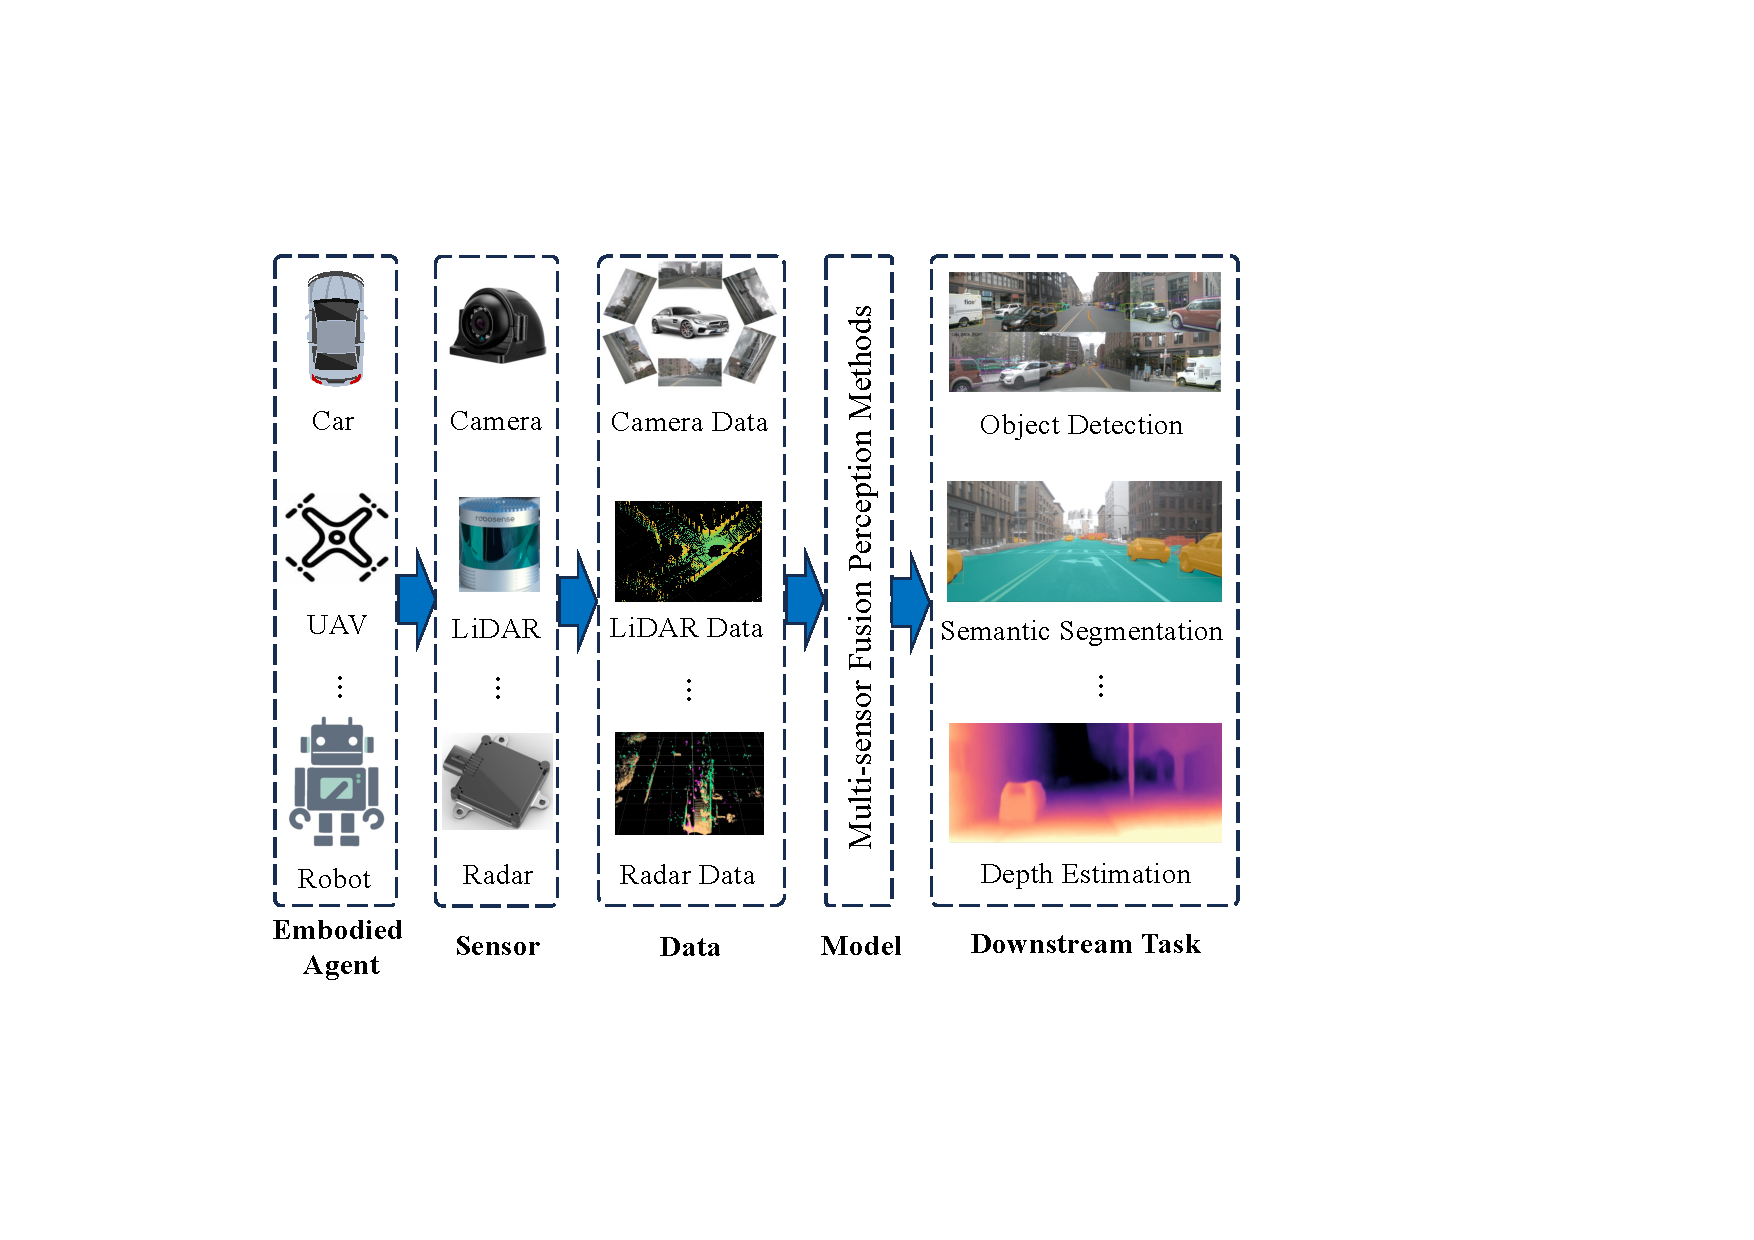
\includegraphics[width=88mm]{figure/MSFP_pipeline.pdf}
    % \vspace{-5mm}
    \caption{Загальна схема конвеєра багатосенсорного сприйняття на основі злиття даних.}
    \vspace{-4mm}
    \label{f:MSFP_pipeline}
\end{figure}

Навколо цих проблем, як показано у табл.~\ref{t:surveys}, за останні роки з'явилися огляди, що систематично узагальнюють відповідні методи~\cite{wangy2023multi,wangl2023multi,xiang2023multi,zhu2023camera,tang2023multi,du2024advancements,bin2024survey,song2024robustness,han2025multimodal}.
Попри значні зусилля, наше детальне дослідження показує, що ці огляди мають низку обмежень.
По-перше, більшість оглядів зорієнтовано на одне завдання або одну дослідницьку область, наприклад, 3D-детектування об'єктів чи автономне керування. Через це дослідники у суміжних задачах часто не можуть скористатися ними напряму.
По-друге, більшість оглядів подають MSFP лише з однієї перспективи мультимодального злиття, не враховуючи різноманітності методів MSFP, як-от мультиагентне злиття та злиття часових рядів.

\begin{table}[t]
    \caption{Огляд споріднених оглядів з MSFP.}
    \label{t:surveys}
    \centering
    \begin{tabular}{m{1.8cm}|m{0.5cm}m{2.4cm}m{2.2cm}}
    \hline
    \textbf{Огляд} & \textbf{Рік}  & \textbf{Область} &\textbf{Завдання}  \\ \hline
   Wang \textit{et al.}~\cite{wangy2023multi}& 2023 &Автономне керування &3D-детектування об'єктів \\
   Wang \textit{et al.}~\cite{wangl2023multi}& 2023 &Автономне керування &3D-детектування об'єктів\\
   Xiang \textit{et al.}~\cite{xiang2023multi}& 2023  &Автономне керування &Не специфіковано\\
   Zhu \textit{et al.}~\cite{zhu2023camera}& 2023 &Не специфіковано  &SLAM\\
   Tang \textit{et al.}~\cite{tang2023multi}& 2023 &Автономне керування  &3D-детектування об'єктів\\
   Du \textit{et al.}~\cite{du2024advancements}& 2024 &Не специфіковано &SLAM\\
   Bin \textit{et al.}~\cite{bin2024survey}& 2024 &Гуманоїдні роботи &Не специфіковано\\
   Song \textit{et al.}~\cite{song2024robustness}& 2024 &Автономне керування &3D-детектування об'єктів\\
   Han \textit{et al.}~\cite{han2025multimodal}& 2025 &Робототехніка &Не специфіковано\\ \hline
    \end{tabular}
    % \vspace{-2mm}
\end{table}


Тож у цій статті ми прагнемо впорядкувати дослідження MSFP з \emph{незалежної від завдання} перспективи, де методи представлено суто з різних технічних поглядів.
Зокрема, ми спочатку вводимо передумови MSFP, включно з різними завданнями сприйняття, різними типами сенсорних даних, поширеними наборами даних та відповідними критеріями оцінювання.
Далі ми розглядаємо методи мультимодального злиття з рівнів окремих точок, вокселів, регіонів та багаторівневого злиття.
Послідовно ми досліджуємо методи мультиагентного злиття, зосереджуючись на спільному (колаборативному) сприйнятті між кількома втіленими агентами та інфраструктурою.
Далі також досліджуються методи злиття часових рядів, які об'єднують часово-впорядковані~(\textit{напр.}, кілька попередніх кадрів) сенсорні дані для прогнозування.
В епоху великих моделей ми досліджуємо методи злиття на основі MM-LLM, поділяючи їх на ``візуально-мовні'' (vision-language) та ``візуально-LiDAR-мовні'' (vision-LiDAR-language); ці методи рідко включалися до попередніх оглядів.
Нарешті, ми всебічно обговорюємо відкриті виклики та майбутні можливості у MSFP на рівнях даних, моделі та застосування.
Сподіваємось, цей огляд допоможе дослідникам зрозуміти важливий поступ у MSFP за останнє десятиліття та надасть відправні точки для майбутніх досліджень.

Решту статті організовано так.
У розділі~\ref{s:background} ми описуємо передумови MSFP з боку різних сенсорних даних, доступних наборів даних і різних завдань сприйняття.
У розділі~\ref{s:multi-modal} ми вводимо методи мультимодального злиття на різних рівнях, \textit{напр.}, рівень окремих точок, вокселів, регіонів і багаторівневий.
У розділі~\ref{s:multi-view} ми підсумовуємо методи мультиагентного спільного сприйняття.
У розділі~\ref{s:time series} ми розглядаємо методи злиття часових рядів для MSFP.
У розділі~\ref{s:MM-LLM} ми досліджуємо сучасні методи MSFP на основі MM-LLM.
У розділі~\ref{s:open challenges} ми обговорюємо відкриті виклики та майбутні напрямки в MSFP.
Нарешті, ми завершуємо нашу роботу в розділі~\ref{s:conclusion}.

\section{Передумови}
\label{s:background}

У цьому розділі ми зосереджуємось на передумовах MSFP. Спершу ми досліджуємо поширені сенсори та їхні типи даних.
Далі систематизуємо доступні дослідникам еталонні набори даних.
Нарешті, докладно описуємо різноманітні низхідні завдання для MSFP.

\subsection{Сенсорні дані}

\subsubsection{Дані з камер}
Камери здатні фіксувати багаті ознаки зовнішнього вигляду об'єктів — кольори, форми та текстури, що є вирішальним для різноманітних завдань сприйняття. Однак, як пасивні сенсори, камери чутливі до умов освітлення. Якість зображення суттєво погіршується вночі та за несприятливої погоди, як-от туман і дощ.

\subsubsection{Дані LiDAR}
LiDAR обчислює відстані до об'єктів, вимірюючи часову різницю між випроміненим і прийнятим лазерним сигналом.
Він безпосередньо видає високоточні 3D-хмари точок, що містять просторову геометричну інформацію, що дає унікальні переваги в 3D-сприйнятті. Втім, він зазвичай чутливий до погоди. Через властиві розрідженість і нерівномірність, ефективне представлення та розуміння хмар точок LiDAR також залишаються складними задачами.

\subsubsection{Дані радарів міліметрового діапазону}
Радари міліметрового діапазону~(mmWave) детектують об'єкти, випромінюючи й приймаючи радіохвилі.
Порівняно з хмарами точок LiDAR, хмари точок радара є розрідженішими й погано описують контури об'єктів. Однак радари зберігають хорошу продуктивність у несприятливих погодних умовах і можуть безпосередньо вимірювати швидкості об'єктів.

\subsection{Набори даних}

\begin{table}[t]
\centering
\caption{Статистика популярних наборів даних для MSFP. Тут L, R, C означають LiDAR, Radar та Camera (камеру) відповідно. U, S, H означають міські, приміські та шосейні умови відповідно.}
\label{tab:3Ddatasets}
\begin{tabular}{l|lllll}
\hline
\textbf{Набір даних} & \textbf{Модальність} & \textbf{Сценарій} & \textbf{\# Класів} & \textbf{\# Кадрів} \\
\hline
KITTI~\cite{geiger2012kitti}  & L + C & U + S + H & 8 & 15K \\
nuScenes~\cite{caesar2020nuscenes}  & L + R + C & U + S & 23 & 1M+ \\
Waymo Open~\cite{sun2020waymo}  & L + R + C & U + S & 4 & 1M+ \\
Cityscapes 3D~\cite{Gahlert2020Cityscapes3D} & C  & U & 30 & 35K \\
Argoverse~\cite{chang2019argoverse} & L + R + C & U & 15 & 1.75M+ \\
A*3D~\cite{pham2020a3d} & L + C  & U & 10 & 100K \\
ApolloScape~\cite{huang2018apolloscape} & L + C & U + S + H & 35 & 140K \\
AIODrive~\cite{weng2020all} & L + R + C  & U & 20 & 500K+ \\
H3D~\cite{patil2019h3d}  & L + C & U & 8 & 60K \\
\hline
\end{tabular}
% \vspace{-2mm}
\end{table}


\subsubsection{KITTI}
KITTI~\cite{geiger2012kitti} складається з $14\,999$ зображень і відповідних хмар точок, з яких $7\,481$ для навчання і $7\,518$ для тестування. Анотації охоплюють вісім категорій та поділяються на прості, середні та складні залежно від розміру, перекриттів і рівнів обрізання.
Транспортний засіб для збору даних мав дві монохромні камери, дві кольорові камери, 64-променевий LiDAR Velodyne, чотири оптичні об'єктиви та GPS-систему. Дані зібрано приблизно з $50$ сцен у Карлсруе та сусідніх німецьких містах, що охоплюють міські, сільські й шосейні умови.


\subsubsection{nuScenes}
NuScenes~\cite{caesar2020nuscenes} було зібрано в Бостоні та Сінгапурі. Містить $700$ тренувальних, $150$ валідаційних і $150$ тестових сцен. Кожна сцена триває приблизно $20$ секунд із $40$ зразками, загалом близько $5{,}5$ годин. Набір містить $1{,}4$ мільйона зображень з камер, $390$~тис.\ сканувань LiDAR, $1{,}4$ мільйона сканувань радара та $1{,}4$ мільйона анотованих обмежувальних рамок у $40$~тис.\ ключових кадрах.
Платформа оснащена $6$ камерами з оглядом 360 градусів, 32-променевим LiDAR з $1{,}39$ мільйона точок на кадр, $5$ радарами міліметрового діапазону та інерціальною навігаційною системою з GPS і IMU.

\subsubsection{Waymo Open}
Waymo Open~\cite{sun2020waymo} містить набори для сприйняття та руху.
Анотації у наборі для сприйняття включають $1{,}26$ мільйона 3D-обмежувальних рамок, $1{,}18$ мільйона 2D-обмежувальних рамок, мітки паноптичної сегментації для $100$~тис.\ зображень, $14$ ключових точок (keypoints) та мітки 3D-семантичної сегментації.
Набір для руху містить $103\,354$ кліпи з траєкторіями об'єктів.
Набір охоплює сценарії денного, нічного, світанкового, сутінкового та дощового часу, проте бракує екземплярів екстремальної погоди.

\subsubsection{Cityscapes 3D}
Cityscapes 3D~\cite{Gahlert2020Cityscapes3D} походить від набору Cityscapes~\cite{Cordts2016Cityscapes}, доповненого анотаціями 3D-обмежувальних рамок.
Він складається з $5$~тис.\ зображень із тонкими анотаціями (\textit{тобто} $2048\times 1024$ пікселів) і $20$~тис.\ зображень з грубими анотаціями, що використовуються для завдань 3D-розуміння сцени міських ландшафтів, \textit{напр.}, семантичної сегментації на рівні екземпляра.

\subsubsection{Argoverse}
Argoverse~\cite{chang2019argoverse} зібрано двома 32-канальними LiDAR-сенсорами, сімома круговими камерами та двома передніми стереокамерами, що охоплюють 360 градусів.
Він містить 3D-набір для трекінгу із $1$~тис.\ 3D-анотованих зразків, що охоплює $30$ категорій об'єктів.
Також містить набір для передбачення руху з $250$~тис.\ зразків з траєкторними даними сцен, $20$~тис.\ неанотованих LiDAR-зразків і $1$~тис.\ карт високої роздільної здатності, що надають багату семантичну анотаційну інформацію щодо дорожньої інфраструктури та правил дорожнього руху.

\subsubsection{A*3D}
A*3D~\cite{pham2020a3d} зібрано переважно на міських дорогах Сінгапуру. Містить понад $39$~тис.\ анотованих кадрів, кожен з яких помічений 2D- та 3D-обмежувальними рамками і має ідентифікатор трекінгу між кадрами. Набір A*3D включає різні сенсорні дані — щільні 3D-хмари точок, RGB-зображення високої роздільної здатності та IMU-дані, що покривають огляд 360 градусів. Він охоплює різні погодні умови (день, ніч, дощ) та різні сценарії збору даних на міських дорогах.


\subsubsection{ApolloScape}
ApolloScape~\cite{huang2018apolloscape} зібрано двома LiDAR-сенсорами, шістьма відеокамерами та системою IMU/GNSS; містить понад $140$~тис.\ зображень високої роздільної здатності. Покриває різні часові інтервали та погодні умови; має загалом $25$ категорій.

\subsubsection{AIODrive}
AIODrive~\cite{weng2020all} розроблено дослідницькою групою Університету Карнегі-Меллона; теж зорієнтовано на міську сцену. Синтетичні сенсорні дані AIODrive включають п'ять RGB-камер $1920 \times 720$ і п'ять камер глибини, один радар, один LiDAR Velodyne-64, IMU, GPS та три далекодійні LiDAR високої щільності.

\subsubsection{H3D}
H3D~\cite{patil2019h3d} зосереджено переважно на 3D-детектуванні та трекінгу об'єктів у міських середовищах. Надає приблизно $160$ міських сцен, зібраних LiDAR Velodyne HDL-64E та трьома RGB-камерами високої роздільної здатності, загалом приблизно $27$~тис.\ кадрів. Кожен кадр містить детальні 3D-обмежувальні рамки та ідентифікатори трекінгу об'єктів.


\subsection{Завдання сприйняття}
\subsubsection{Детектування об'єктів}
Детектування об'єктів — одне з фундаментальних завдань широких систем сприйняття; його основна мета — точно локалізувати та ідентифікувати різні типи об'єктів за даними сенсорів.
У 2D-детектуванні система повинна видавати інформацію про категорію об'єкта та 2D-обмежувальну рамку, представлену як $(x, y, w, h)$.
У сценарії 3D-детектування результати детектування мають включати 3D-координати позиції $(x, y, z)$, інформацію про 3D-розмір $(l, w, h)$ та кут орієнтації~(курс) $\theta$ цілі.

\subsubsection{Семантична сегментація}
Завдання семантичної сегментації полягає у тому, щоб класифікувати кожну базову одиницю сцени, наприклад піксель зображення, в одну із семантичних категорій.
Зокрема, для вхідного набору даних (\textit{напр.}, множини пікселів зображення $\bm{I} = \{\bm{I}_1, \bm{I}_2, ..., \bm{I}_n\}$) і попередньо визначеної множини семантичних категорій $\bm{y} = \{y_1, y_2, ..., y_k\}$, модель сегментації повинна призначити кожній базовій одиниці $\bm{I}_i$ відповідну семантичну мітку або розподіл імовірностей класів.

\subsubsection{Оцінювання глибини}
Оцінювання глибини має на меті отримати інформацію про глибину сцени за сенсорними даними та надати втіленим агентам 3D-геометричне розуміння. За заданим вхідним зображенням $\bm{I} \in \mathcal{R}^{M\times N}$ і відповідною розрідженою картою глибини $\bm{D}_{s} \in \mathcal{R}^{M\times N}$ система оцінювання глибини повинна видати щільну карту глибини $\bm{D}_{d}$, де процес доповнення глибини можна представити як відображення $\bm{D}_d=f(\bm{I}, \bm{D}_{s})$. Через оцінювання глибини система здатна отримати точну 3D-інформацію про положення об'єктів у сцені, що критично важливо для низхідних завдань, як-от планування шляху та керування рішеннями.

\subsubsection{Передбачення зайнятості}
Передбачення зайнятості (occupancy prediction) забезпечує насичене семантичне розуміння 3D-простору. Дискретизуючи неперервний 3D-простір у воксельну ґратку, модель сприйняття зайнятості може передбачити стан зайнятості та семантичну категорію кожного вокселя, надаючи повне представлення сцени для автономних рішень.

\section{Методи мультимодального злиття}
\label{s:multi-modal}

\begin{table}[t]
    \centering
    \caption{Класифікація методів мультимодального злиття для MSFP.}
    \label{t:multi-modal}
    \scalebox{0.9}{\begin{tabular}{m{1.4cm}|m{3.5cm}|m{3.5cm}}
       \hline
       \textbf{Категорія}  & \textbf{Особливість} & \textbf{Методи} \\ \hline
         Злиття на рівні точок & Інтегрують геометричні координати точок LiDAR із семантичними деталями зображень на рівні окремих точок. & PointFusion~\cite{xu2018pointfusion}, PointPainting~\cite{vora2020pointpainting}, MVP~\cite{yin2021multimodal}, DeepFusion~\cite{li2022deepfusion} \\ \hline
         Злиття на рівні вокселів & Перетворюють нерегулярні хмари точок LiDAR на регулярні воксельні ґратки для ефективної обробки; зберігають геометричну інформацію, водночас інтегруючи мультимодальні дані для підвищення семантичного багатства. & CenterFusion~\cite{nabati2021centerfusion}, PointAugmenting~\cite{wang2021pointaugmenting}, UVTR~\cite{li2022unifying}, SFD~\cite{wu2022sparse} \\ \hline
         Злиття на рівні регіонів & Агрегують специфічні для регіону ознаки між модальностями через просторове вирівнювання, використовуючи міжмодальні просторові відповідності з пізнім злиттям. & AVOD~\cite{ku2018joint}, RoarNet~\cite{shin2019roarnet}, AR-CNN~\cite{zhang2019weakly}, E2E-MFD~\cite{zhang2024e2e}\\ \hline
         Багаторівневе злиття & Поєднують мультимодальне злиття на кількох ієрархічних рівнях, використовуючи такі техніки, як багатоетапне злиття, увага або контрастне навчання, для підвищення стійкості сприйняття. & MVX-Net~\cite{sindagi2019mvx}, RCBEV~\cite{zhou2023bridging}, MBNet~\cite{zhou2020improving}, CSSA~\cite{cao2023multimodal}\\ \hline
    \end{tabular}}
\end{table}

Зливаючи дані мультимодальних сенсорів, втілені агенти можуть зменшити сліпі плями сприйняття та досягти комплекснішого сприйняття середовища.
Наприклад, LiDAR забезпечує точну інформацію про глибину, тоді як камери зберігають більше детальної семантичної інформації.
Тому питання, як краще зливати мультимодальні дані з різних сенсорів задля точнішого і стійкішого сприйняття, стало гарячою темою досліджень у численних застосуваннях.
Як показано в табл.~\ref{t:multi-modal}, у цьому розділі ми представляємо різні методи з точки зору різних рівнів злиття, \textit{тобто} рівня точок, вокселів, регіонів та багаторівневого.

\begin{figure}[t]
    \centering
    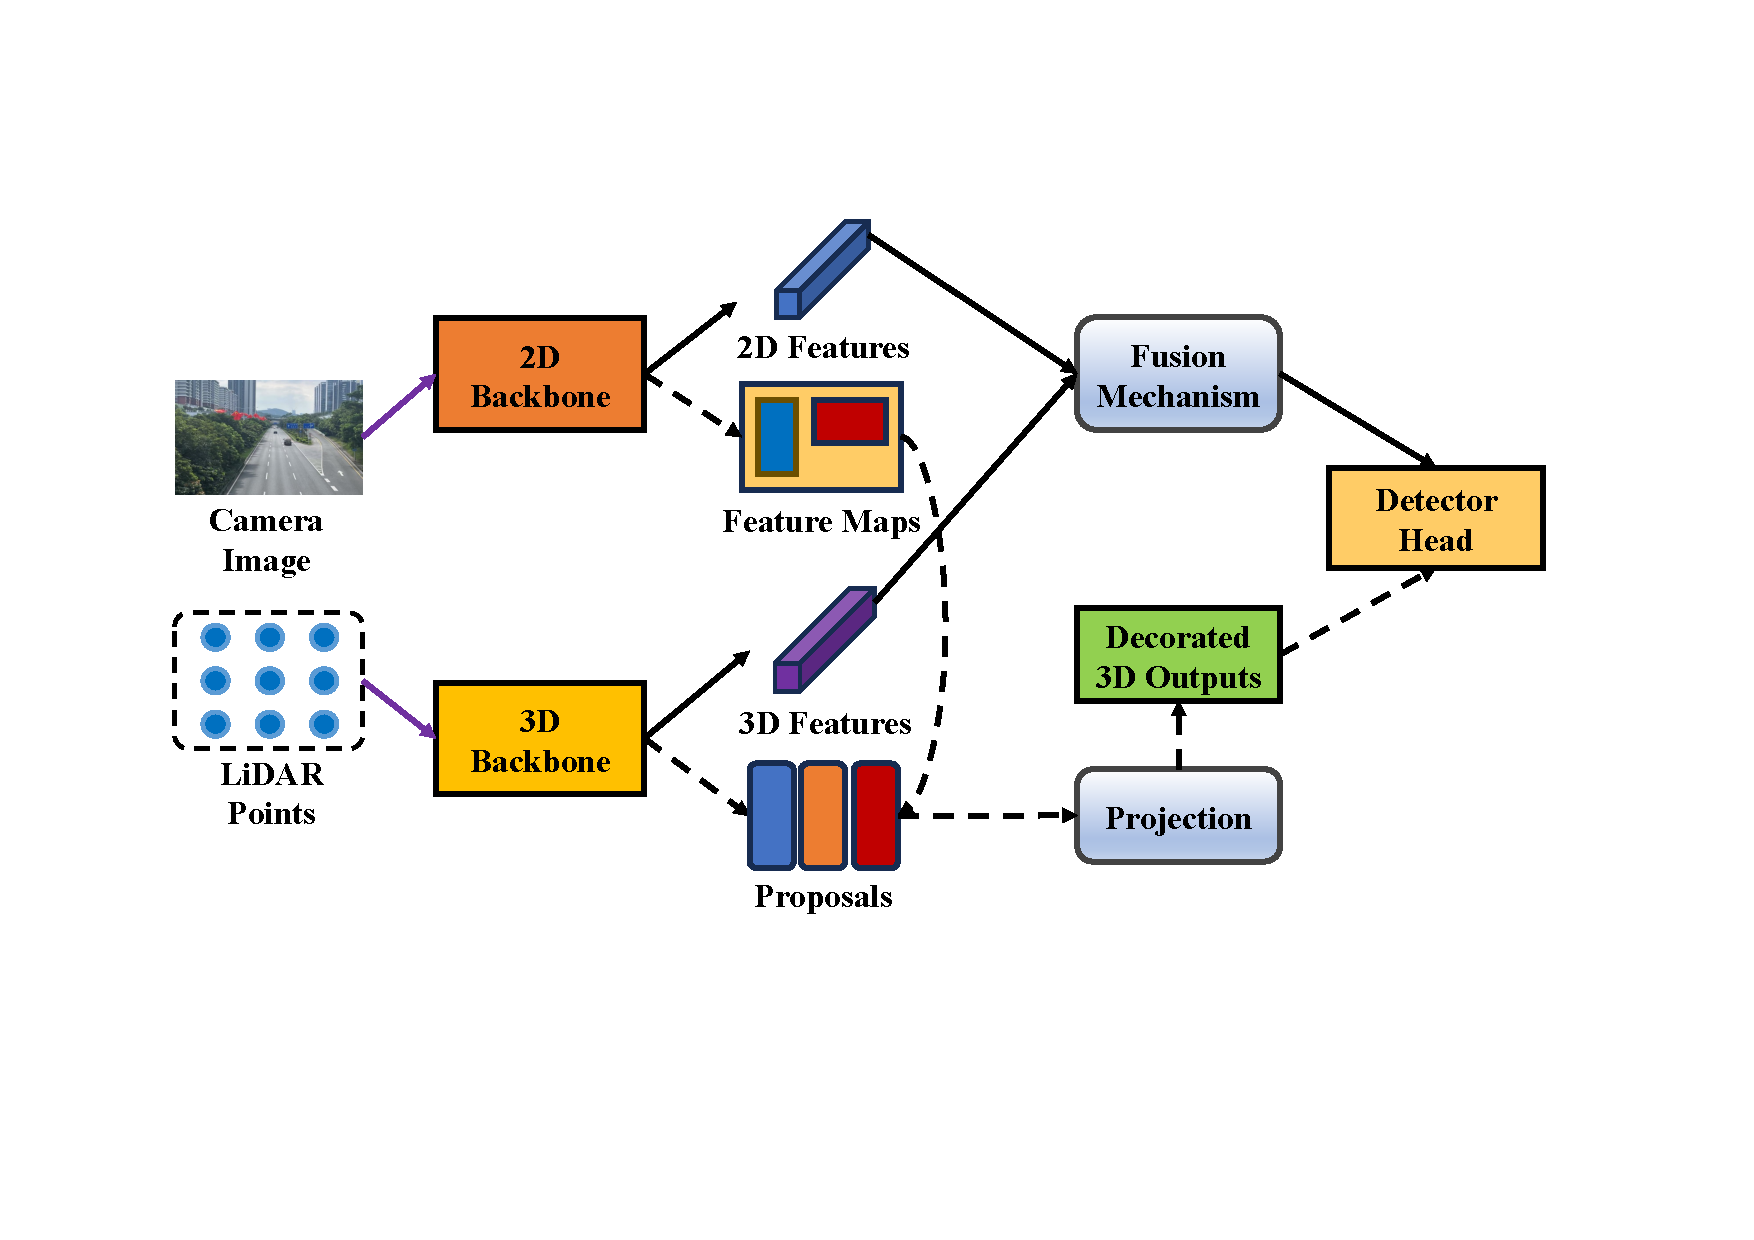
\includegraphics[width=88mm]{figure/point-level.pdf}
    \caption{Загальна схема конвеєра злиття на рівні точок.}
    \label{f:point}
\end{figure}

\subsection{Злиття на рівні точок}
\label{ss:3.2}

Рис.~\ref{f:point} показує типовий конвеєр методів злиття на рівні точок, які мають на меті досягти злиття ознак на рівні окремих точок між хмарами точок LiDAR і даними зображень. Інтегруючи геометричну координатну інформацію хмар точок із семантичними деталями зображень (\textit{напр.}, кольори та категорійні атрибути), можна підвищити точність мультимодального сприйняття.
Серед різних методів, PointNet~\cite{qi2017pointnet} та PointNet++~\cite{qi2017pointnet++} спочатку обробляли хмари точок безпосередньо, не покладаючись на інші форми представлення, як-от воксели. Вони використовувалися лише для розпізнавання 3D-об'єктів на основі LiDAR.
Frustum PointNets~\cite{qi2018frustum} розширює PointNet, перетворюючи 2D-кандидатські рамки на 3D-зрізані піраміди (frustums) і виконуючи сегментацію й регресію безпосередньо на сирих хмарах точок.
PointFusion~\cite{xu2018pointfusion} застосовує стандартніший підхід, окремо витягаючи ознаки з RGB-зображень і хмар точок за допомогою CNN та PointNet відповідно, а потім конкатенуючи їх для злиття.

Однак це початкове злиття погано вловлює складні крос-модальні зв'язки. PI-RCNN~\cite{xie2020pi} вдосконалює це двостадійним процесом, використовуючи увагу (attentive aggregation) для уточнення злиття 3D-пропозицій і 2D-семантичних ознак, що дає змогу детальнішої обробки.
Методи, як-от PointPainting~\cite{vora2020pointpainting} і FusionPainting~\cite{xu2021fusionpainting}, анотують кожну точку LiDAR ознаками зображення: перший проектує точки LiDAR на маски сегментації, другий використовує адаптивну увагу для злиття на семантичному рівні. Ці підходи краще опрацьовують розрідженість хмар точок, ніж методи з пріоритетом пропозицій, як-от PI-RCNN. Аналогічно, MVP~\cite{yin2021multimodal} збагачує розріджені хмари точок, проектуючи результати 2D-детектування у віртуальні 3D-точки та зливаючи їх із даними LiDAR, компенсуючи обмеження LiDAR у детектуванні малих або віддалених об'єктів.
DeepFusion~\cite{li2022deepfusion} застосовує механізм перехресної уваги для динамічного вирівнювання ознак LiDAR і зображень і розв'язує проблеми геометричного розузгодження через зворотну аугментацію даних. GraphAlign~\cite{song2023graphalign} далі оптимізує процес вирівнювання шляхом графового зіставлення ознак. Він досягає точного зіставлення на рівні пікселів між геометричними ознаками хмари точок і семантичними ознаками зображень через модулі вирівнювання графових ознак та самоуваги, розв'язуючи ключові проблеми неточних геометричних позицій та неоднозначних семантичних асоціацій у мультимодальному злитті.


\subsection{Злиття на рівні вокселів}
\label{ss:3.3}

Методи злиття на рівні вокселів перетворюють нерегулярні хмари точок LiDAR на регулярні ґратки (\textit{напр.}, воксели або стовпці-pillars), що дозволяє ефективну обробку зі збереженням геометричної інформації. Рис.~\ref{f:voxel} показує типовий конвеєр методів злиття на рівні вокселів.
Для використання семантичного багатства зображень, зображення камер інтегруються у методи на основі вокселів для покращення сприйняття, особливо у розріджених або зайнятих сценаріях.

Щоб подолати такі проблеми, як неточна інформація про висоту, CenterFusion~\cite{nabati2021centerfusion} розширює радарні точки у 3D-стовпці й асоціює радарні детектування з об'єктами на зображеннях. Однак методи на рівні вокселів часто страждають на ``розмиття ознак'' через втрату просторової інформації всередині вокселя. VPFNet~\cite{zhu2022vpfnet} пом'якшує це, використовуючи шар воксельного RoI-пулінгу та віртуальні точки для вирівнювання та агрегації ознак з LiDAR і зображень. PointAugmenting~\cite{wang2021pointaugmenting} збагачує точки LiDAR ознаками зображень і вокселізує доповнену хмару точок. Однак проектування 3D-точок на площину зображення може погіршити продуктивність в зайнятих ділянках. VFF~\cite{li2022voxel} вводить метод проектування ``точка-в-промінь'' (point-to-ray), зливаючи ознаки зображення вздовж променів задля забезпечення багатшого контекстуального інформаційного супроводу — особливо корисно для детектування зайнятих та віддалених об'єктів.

\begin{figure}[t]
    \centering
    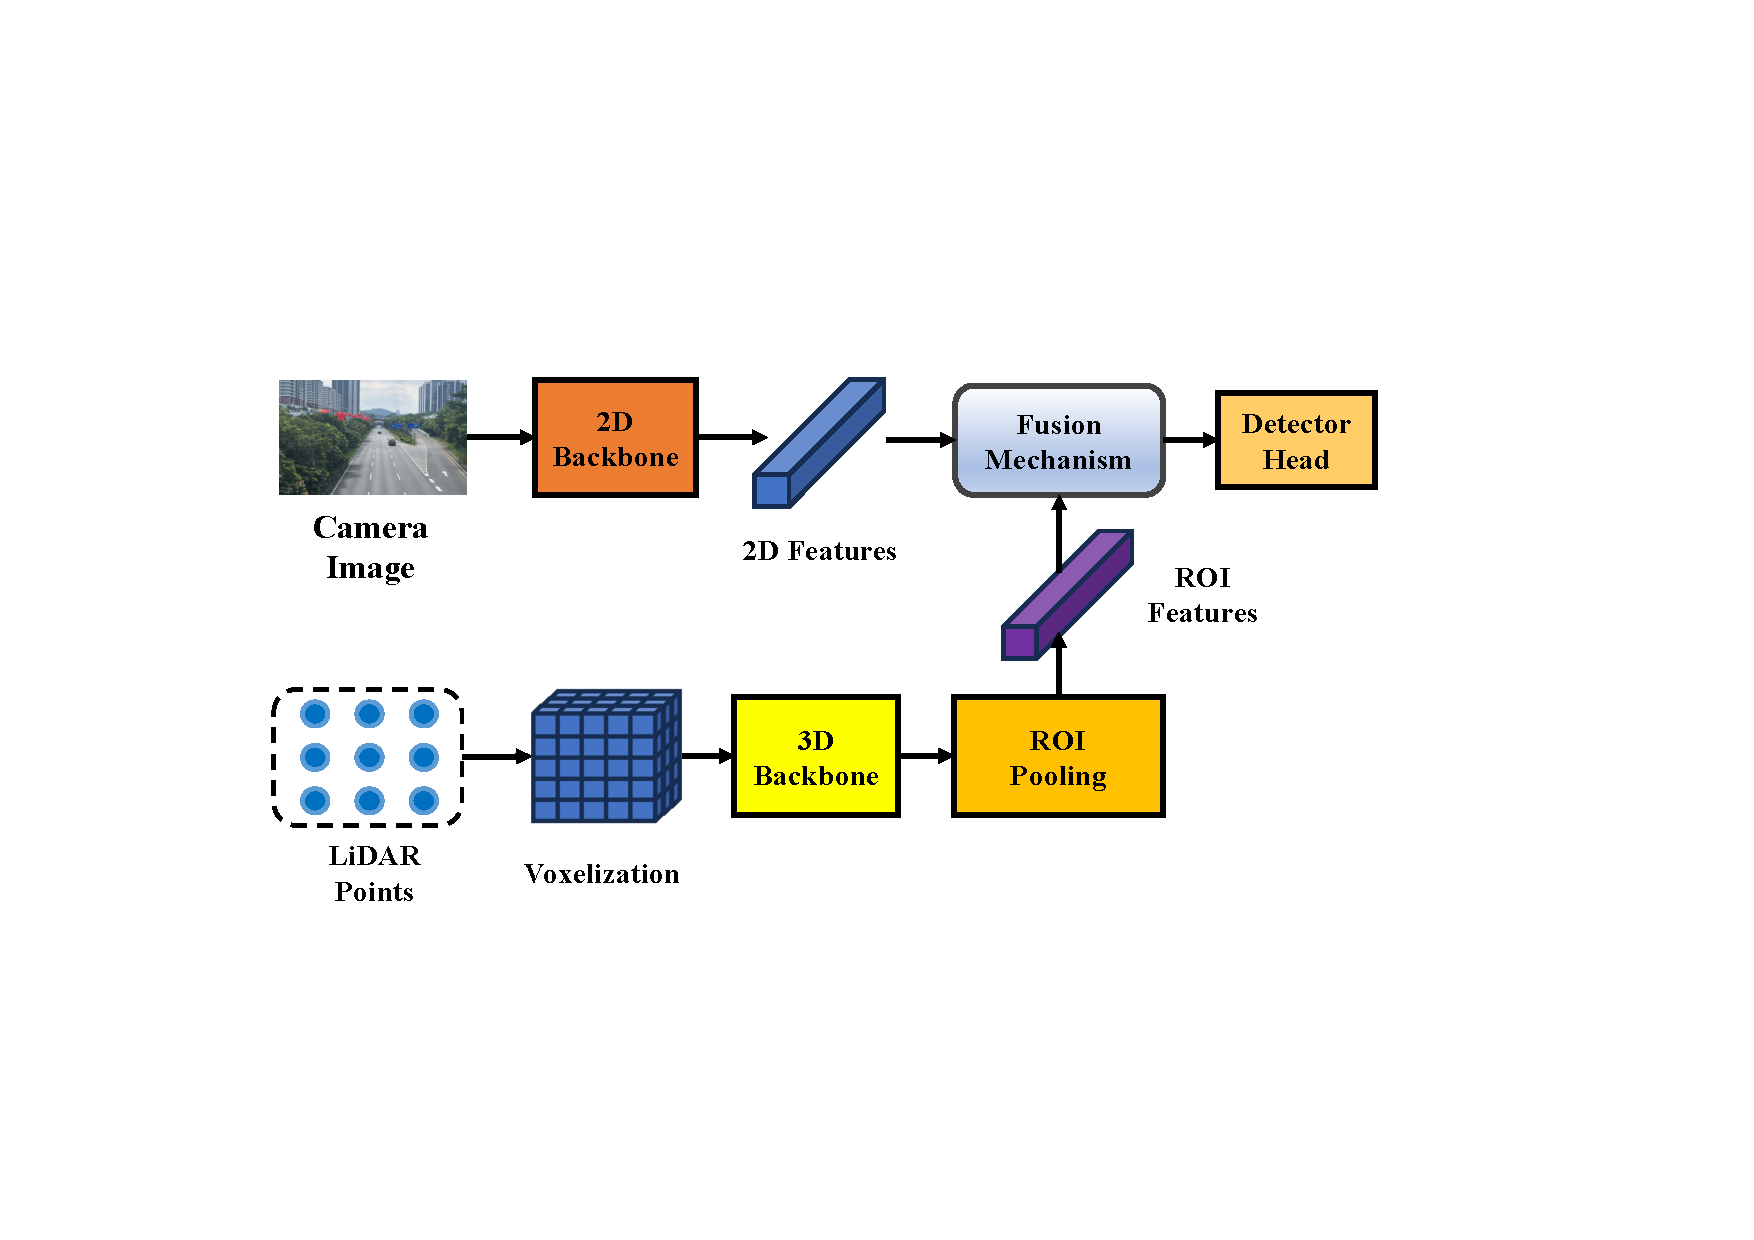
\includegraphics[width=80mm]{figure/voxel-level.pdf}
    \caption{Загальна схема конвеєра злиття на рівні вокселів.}
    \label{f:voxel}
\end{figure}


Для вирівнювання ознак, AutoAlign~\cite{chen2022autoalign} вводить навчальний мультимодальний каркас злиття, динамічно вирівнюючи ознаки зображень і хмар точок без покладання на проекційну матрицю. Як покращена версія AutoAlign, AutoAlignV2~\cite{chen2022deformable} використовує деформівну увагу та розріджену вибірку для підвищення ефективності та зниження обчислювальних витрат, водночас спрощуючи аугментацію даних порівняно з ранішими методами, як-от PointAugmenting. VoxelNextFusion~\cite{song2024voxelnextfusion} поєднує воксельні ознаки з відповідними та оточуючими піксельними ознаками за допомогою самоуваги для злиття точок і блоків. Цей підхід ефективно розв'язує невідповідності роздільної здатності та покращує детектування далеких і складних об'єктів.

\subsection{Злиття на рівні регіонів}
\label{ss:3.4}

Методи злиття на рівні регіонів зосереджуються на агрегації специфічної для регіонів інформації, такої як карти ознак, ROI (область інтересу) або регіональні пропозиції, з 2D-зображень та інших модальностей. Ці методи особливо ефективні у сценаріях, де просторове вирівнювання між модальностями досягти простіше.
AVOD~\cite{ku2018joint} ввів мультимодальну мережу пропозицій регіонів, яка обробляє BEV- та RGB-зображення окремо для генерації карт ознак високої роздільної здатності. Регресуючи вектори напрямку, AVOD розв'язує неоднозначність у визначенні напрямку. Аналогічно, RoarNet~\cite{shin2019roarnet} застосовує двостадійний каркас: перша стадія передбачає 3D-пози безпосередньо із зображень для уникнення втрати інформації, пов'язаної з проекцією, а друга стадія уточнює ці передбачення з використанням міркувань про хмару точок. TransFusion~\cite{bai2022transfusion} використовує трансформери для злиття LiDAR-camera, встановлюючи м'які асоціації між точками LiDAR і пікселями зображень. Він адаптується до контекстуальної інформації, розв'язуючи проблеми стійкості, спричинені поганою якістю зображення або помилками калібрування сенсорів.

\begin{figure}[t]
    \centering
    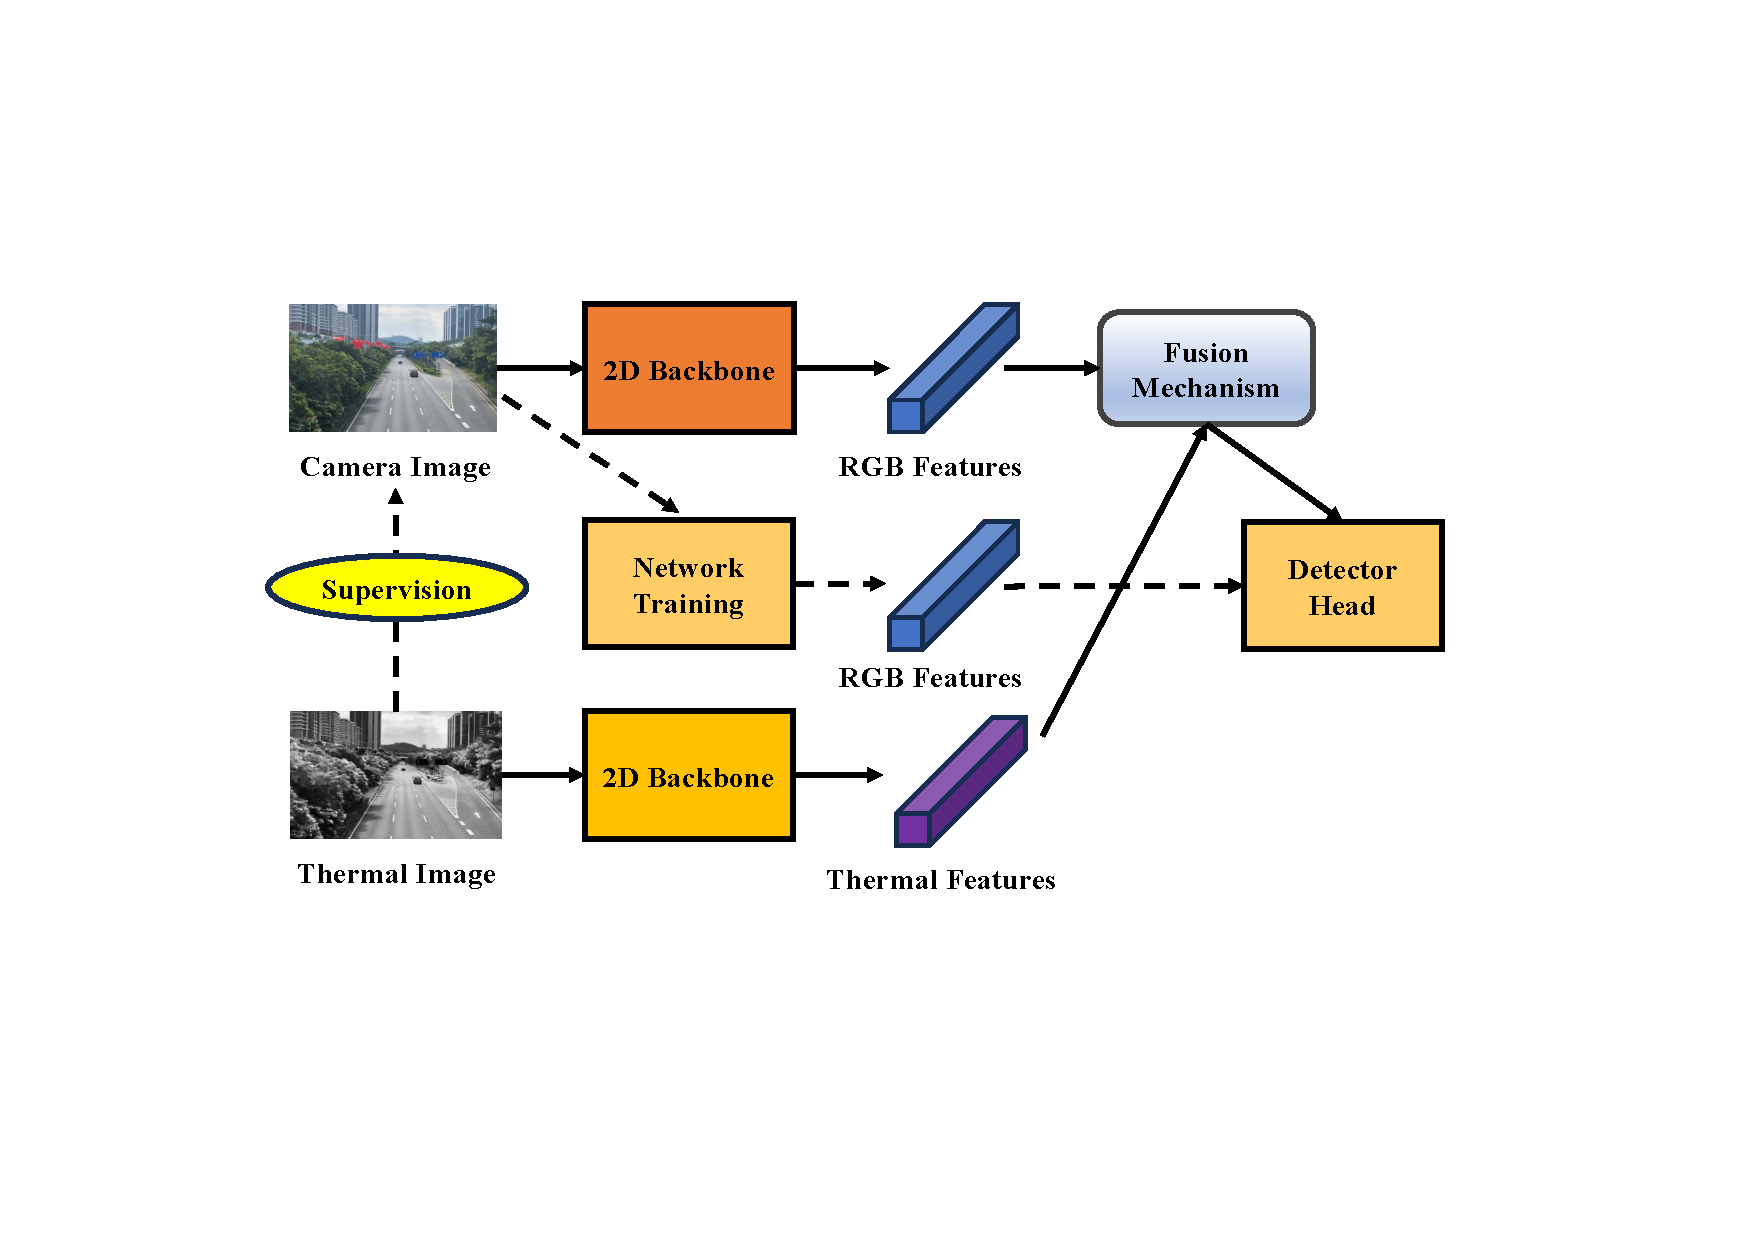
\includegraphics[width=80mm]{figure/region-level.pdf}
    \caption{Загальна схема конвеєра злиття на рівні регіонів.}
    \label{f:region}
\end{figure}

Для злиття термальних і RGB-зображень методи на рівні регіонів є поширенішими через простіше вирівнювання ознак.
Рис.~\ref{f:region} відображає конвеєр методів злиття на рівні регіонів. CMT-CNN~\cite{xu2017learning} вирішує задачу детектування пішоходів за умов слабкого освітлення, реконструюючи термальні регіони, що відповідають RGB-кандидатським регіонам, і зливаючи крос-модальну інформацію через мультимасштабну мережу детектування. AR-CNN~\cite{zhang2019weakly} розв'язує розузгодження між RGB- та термальними зображеннями, передбачаючи позиційні зсуви та адаптивно вирівнюючи регіональні ознаки. Двопотокові архітектури, як-от GAFF~\cite{zhang2021guided} і RSDet~\cite{zhao2024removal}, обробляють RGB- і термальні зображення окремо перед злиттям ознак. GAFF використовує внутрішньо- та міжмодальні механізми уваги для вибору ознак, а RSDet уточнює злиття через видалення надмірних спектрів та динамічний вибір ознак.

\subsection{Багаторівневе злиття}
\label{ss:3.5}

Багаторівневе злиття інтегрує мультимодальну інформацію з різних рівнів для забезпечення комплекснішого сприйняття.
Рис.~\ref{f:multi} ілюструє конвеєр методів багаторівневого злиття.
У літературі Liang \textit{et al.}~\cite{liang2018deep} використовують неперервні згортки для злиття карт ознак зображень і LiDAR на різних рівнях у просторі BEV.
Zhu \textit{et al.}~\cite{zhu2021cross} представляють двостадійний метод крос-модального злиття, що збагачує семантичне багатство та локальне представлення пропозицій з рівня точок і рівня регіонів. У такий спосіб продуктивність сприйняття можна покращити у сценаріях з розрідженістю та зайнятістю.
Аналогічно, MVX-Net~\cite{sindagi2019mvx} виконує злиття на рівні точок і на рівні вокселів. MMF~\cite{liang2019multi} розширює цю ідею до багатозадачного каркасу, як-от 2D/3D-детектування, оцінювання поверхні та доповнення глибини.

Для підвищення стійкості, EPNet~\cite{huang2020epnet} вводить модуль LI-Fusion, що знижує вплив нерелевантної інформації, зливаючи ознаки зображень і хмар точок на різних масштабах.
Як покращена версія, EPNet++~\cite{liu2022epnet++} також вводить двонапрямну взаємодію інформації: ознаки хмари точок використовуються для уточнення ознак зображень, і навпаки.
У такий спосіб EPNet++ досягає стійкішого представлення ознак. RCBEV~\cite{zhou2023bridging} зосереджується на сприйнятті динамічних об'єктів, перекидаючи місток між відмінностями ознак радара та камери; а
DVF~\cite{mahmoud2023dense} збагачує представлення у ділянках низької щільності шляхом генерації багатомасштабних щільних воксельних ознак, уникаючи зашумлених 2D-передбачень з мітками 3D-обмежувальних рамок.
LoGoNet~\cite{li2023logonet} поєднує глобальне і локальне злиття з динамічною агрегацією ознак задля підвищення точності детектування у складних середовищах.

Деякі сучасні методи застосовують механізми уваги та контрастне навчання для збагачення мультимодального злиття. Наприклад, CAT-Det~\cite{zhang2022cat} кодує глобальну контекстуальну інформацію між модальностями за допомогою контрастного навчання. SeaDATE~\cite{dong2024seadate} використовує подвійну увагу та контрастне навчання для витягання глибокої семантичної інформації, тоді як CSSA~\cite{cao2023multimodal} застосовує легке перемикання каналів та просторову увагу для ефективного злиття. Fusion-Mamba~\cite{dong2024fusion} розв'язує задачу вирівнювання через покращену структуру Mamba та простір прихованих станів.

\begin{figure}[t]
    \centering
    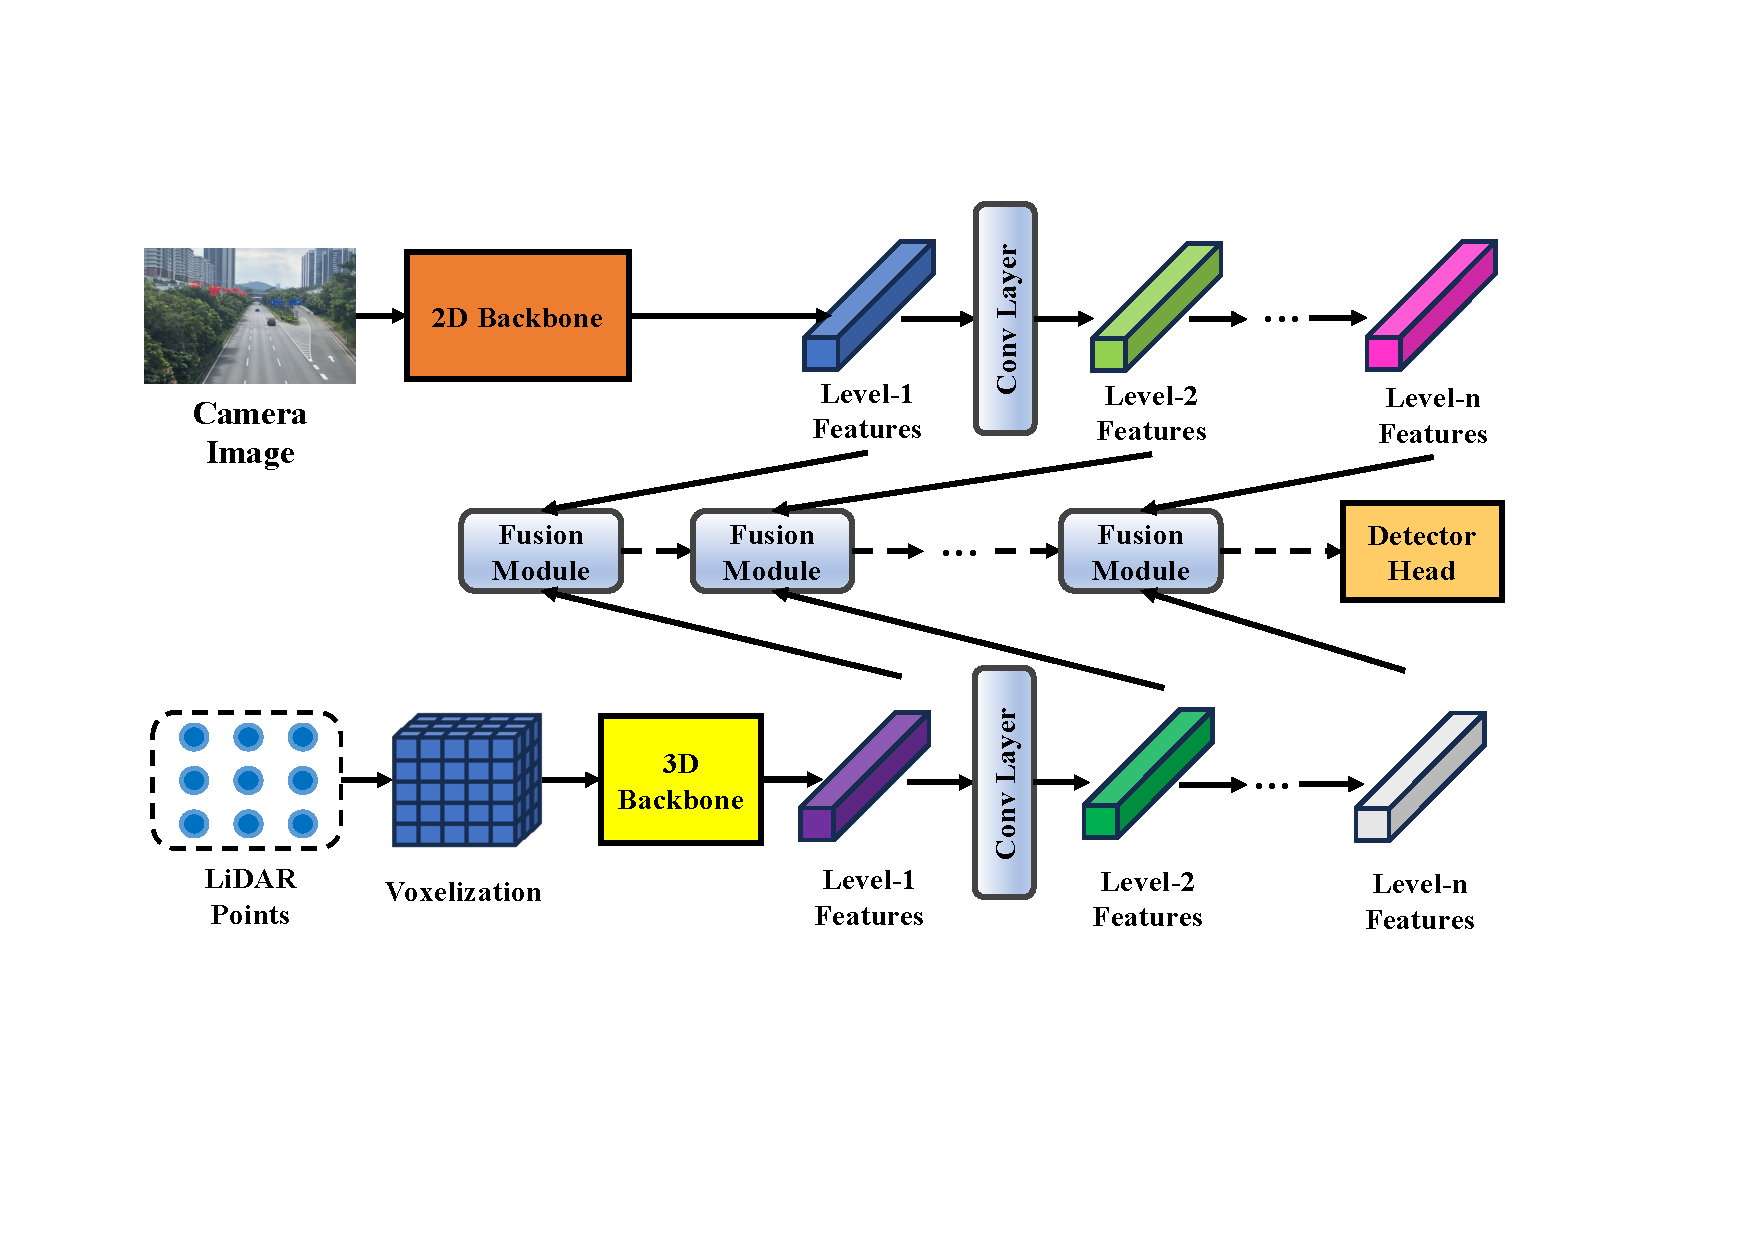
\includegraphics[width=85mm]{figure/multi-level.pdf}
    \caption{Конвеєр багаторівневого злиття.}
    \label{f:multi}
\end{figure}

\section{Методи мультиагентного злиття}
\label{s:multi-view}

У складних відкритих середовищах, особливо за обмеженої видимості або несприятливої погоди, система сприйняття одного втіленого агента стикається з численними викликами.
Технологія спільного (колаборативного) сприйняття може інтегрувати дані сприйняття з кількох агентів та інфраструктури, що є вирішальним для подолання проблем перекриттів та відмов сенсорів.
У цьому розділі ми зосереджуємось на багатовидовому злитті в режимі агент-до-агента~(agent-to-agent, A2A) спільного сприйняття.
Рис.~\ref{f:agent} показує простий конвеєр злиття A2A.

CoBEVT~\cite{xu2022cobevt} — перший універсальний мультиагентний мультикамерний каркас сприйняття. Він генерує BEV-передбачення сегментації через розріджені трансформери для спільного оброблення. CoBEVT містить модуль осьової уваги (axial attention) для ефективного злиття мультиагентних мультивидових ознак камер, охоплюючи як локальні, так і глобальні просторові взаємодії.
CoCa3D~\cite{hu2023collaboration} пропонує інноваційний спільний каркас з виключно камерним сприйняттям. Він розв'язує проблему упередженості передбачення глибини, дозволяючи кільком агентам, обладнаним лише камерами, ділитися візуальною інформацією. Через спільне використання інформації про глибину в однакових точках CoCa3D зменшує помилки, краще опрацьовує невизначеності глибини та розширює можливості детектування на зайняті та далекодійні зони, які зазвичай складні для одноагентних систем.
V2VNet~\cite{wang2020v2vnet} вводить каркас на основі графових нейронних мереж для злиття проміжних представлень ознак від кількох транспортних засобів.
MACP~\cite{ma2024macp} досліджує ефективну адаптацію моделей з використанням попередньо натренованих одноагентних моделей задля досягнення спільного сприйняття з малою кількістю параметрів та комунікаційних витрат.
HM-ViT~\cite{xiang2023hm} пропонує уніфікований каркас для проблеми мультимодального A2A-сприйняття, здатний зливати мультивидові ознаки зображень та хмар точок LiDAR з різних типів сенсорів, забезпечуючи ефективне мультимодальне кооперативне сприйняття.
MRCNet~\cite{hong2024multi} вирішує проблеми розмиття руху (motion blur), вводячи механізм підсилення руху, який зменшує вплив розмиття руху на детектування об'єктів через захоплення контексту руху, досягаючи кращих результатів у зашумлених сценаріях.

Окрім того, деякі роботи зосереджуються на покращенні комунікаційних аспектів спільного сприйняття задля ефективнішої та стійкішої кооперації. When2Com~\cite{liu2020when2com} запропонував каркас навчання тому, як формувати комунікаційні групи і коли комунікувати. Використовуючи механізми ``рукостискання'' (handshake) та асиметричні розміри повідомлень, він зменшує використання пропускної здатності та досягає хороших результатів у завданнях семантичної сегментації та розпізнавання 3D-форм. Who2Com~\cite{liu2020who2com} підвищує точність у завданнях семантичної сегментації через навчання механізмів handshake-комунікації та використовує меншу пропускну здатність порівняно з централізованими методами. How2Com~\cite{yang2024how2comm} додатково запропонував комунікаційний механізм на основі теорії інформації та просторово-часовий спільний трансформер, що покращує спільне сприйняття через фільтрування ознак, компенсацію затримок та просторово-часове злиття, що дає ефективнішу та стійкішу кооперацію у задачах 3D-детектування об'єктів.
CodeFilling~\cite{hu2024communication} ефективно оптимізує представлення та вибір спільних повідомлень через стратегію заповнення інформацією та техніки кодокнижкового стиснення, досягаючи ефективного спільного сприйняття з низькими комунікаційними витратами.

\begin{figure}[t]
    \centering
    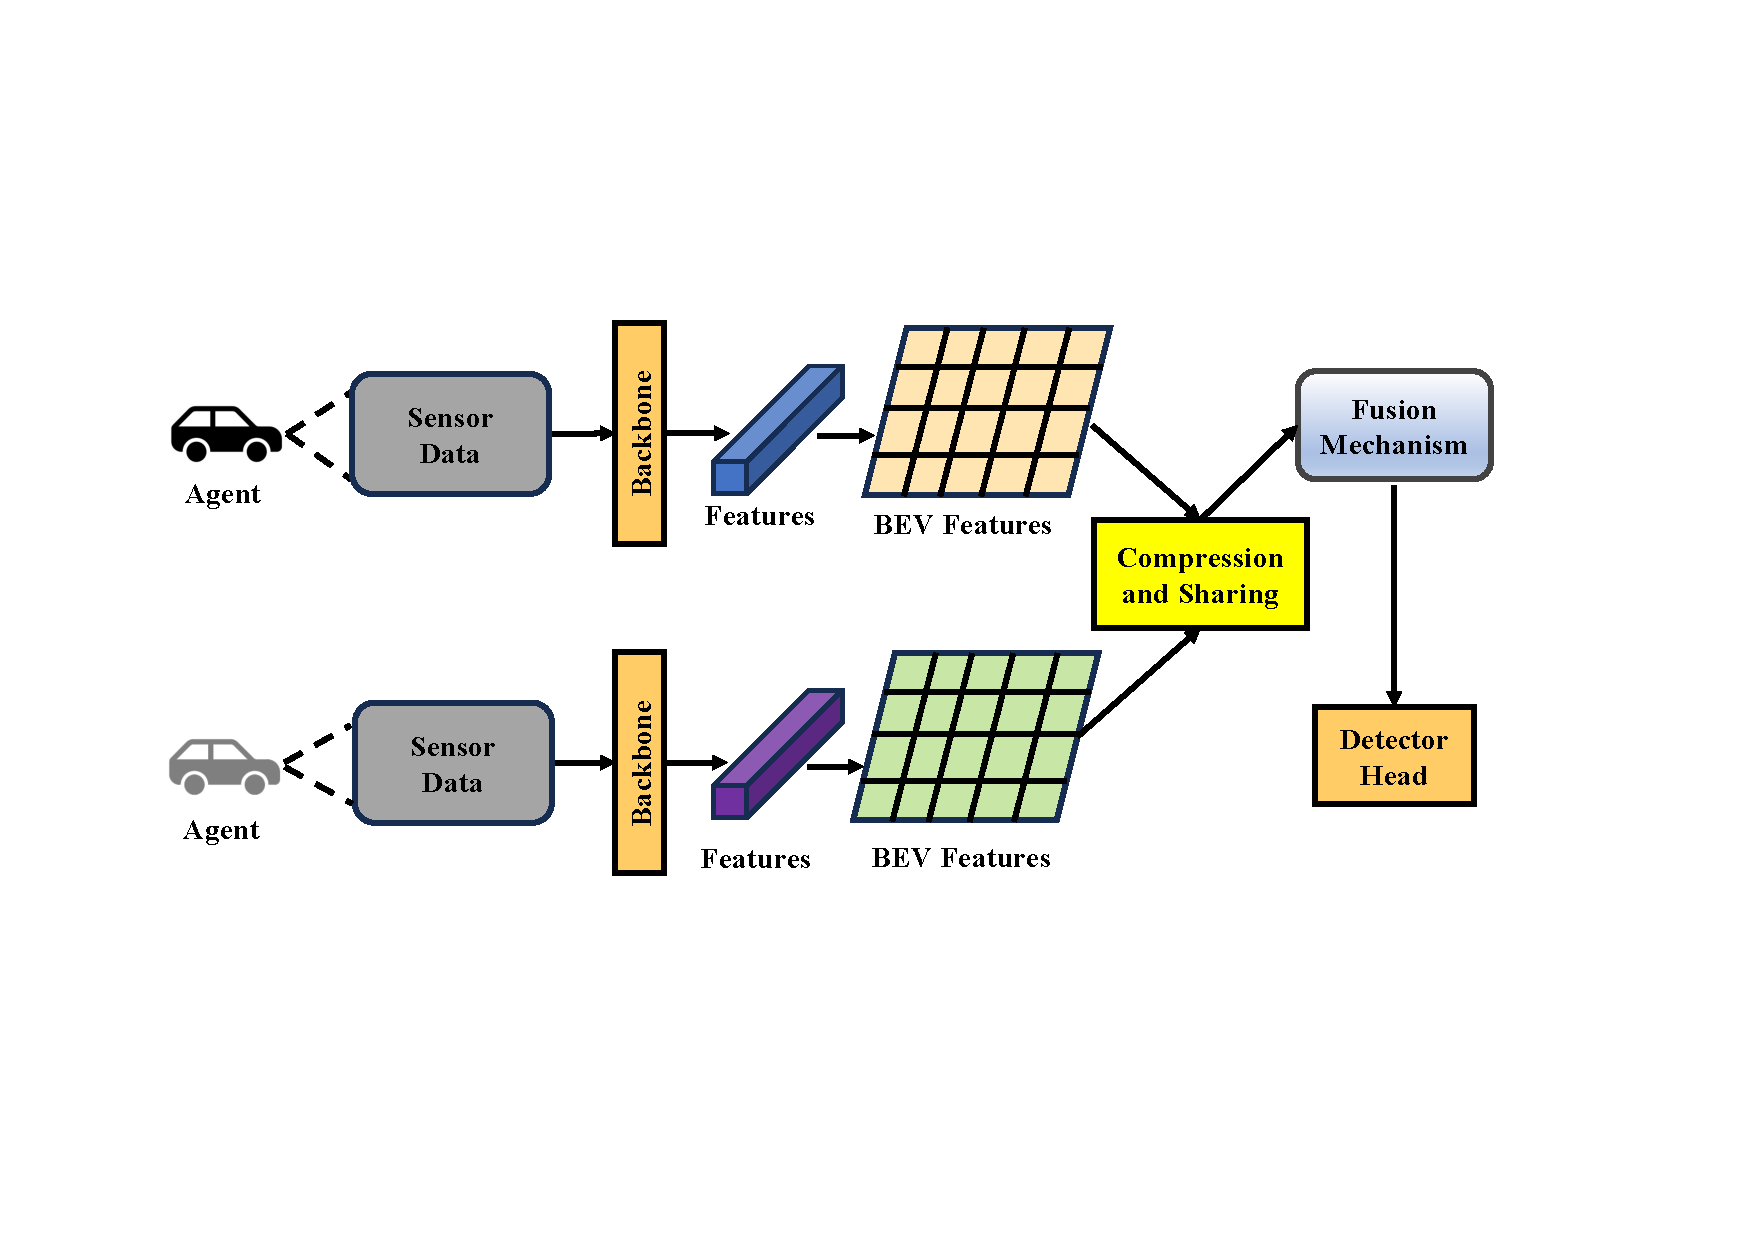
\includegraphics[width=85mm]{figure/multi-agent.pdf}
    \caption{Простий конвеєр злиття агент-до-агента~(A2A).}
    \label{f:agent}
\end{figure}

\section{Злиття часових рядів}
\label{s:time series}

Злиття часових рядів є критичним складником систем MSFP: воно долає обмеження окремого кадру та збагачує перцептивну неперервність у просторово-часових доменах.
Рис.~\ref{f:time_series_frame} показує простий конвеєр такого злиття.
З появою трансформерних архітектур у комп'ютерному зорі переважними стали методи на основі запитів (query-based), де ознаки сприйняття, закодовані як запити, взаємодіють з просторово-часовими ключами та значеннями для досягнення ефективного вирівнювання ознак.
Як показано в табл.~\ref{t:time-series}, ці методи можна класифікувати на три основні категорії: \textit{щільні запити}, \textit{розріджені запити} та \textit{гібридні запити}.
Рис.~\ref{f:time-series-timeline} зображує часову лінію query-методів для злиття часових рядів багатосенсорних даних.

\begin{figure}[t]
    \centering
    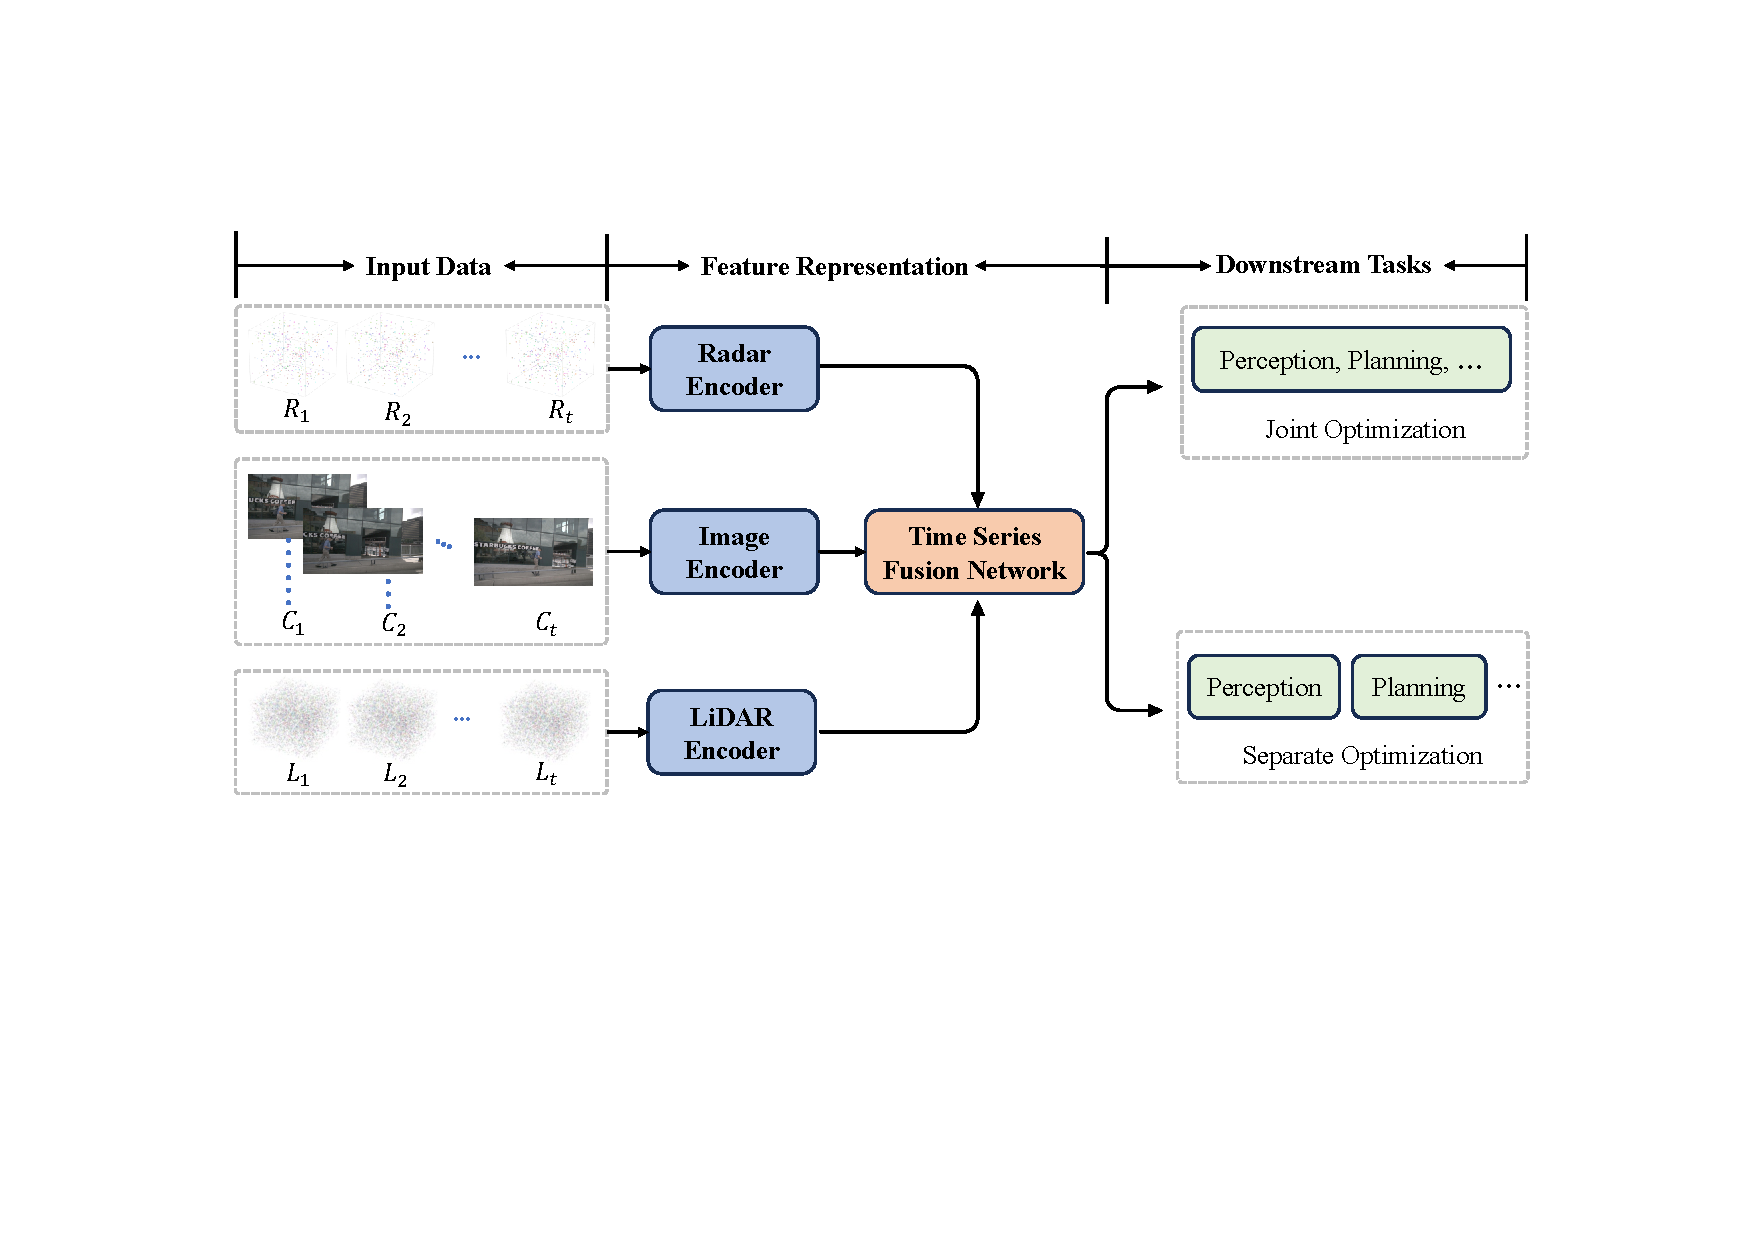
\includegraphics[width=85mm]{figure/time-series-fusion.pdf}
    \caption{Загальний огляд каркасу мережі для злиття часових рядів багатосенсорних даних.}
    % \vspace{-4mm}
    \label{f:time_series_frame}
\end{figure}

\begin{table}[t]
    \centering
    \caption{Класифікація методів злиття часових рядів на основі запитів.}
    \label{t:time-series}
    \scalebox{0.96}{
    \begin{tabular}{m{1cm}|m{3.3cm}|m{3.3cm}}
       \hline
       \textbf{Категорія}  & \textbf{Особливість} & \textbf{Методи} \\ \hline
         Щільні запити & Зберігають фіксовані просторові позиції у просторах представлення високої роздільної здатності & BEVFormer~\cite{li2022bevformer}, BEVFormer v2~\cite{yang2023bevformer} \\ \hline
         Розріджені запити & Ефективно концентрують обчислювальні ресурси на областях інтересу & StreamPETR~\cite{streampetr}, Sparse4D (v1~\cite{2211.10581}/v2~\cite{lin2023sparse4d}/v3~\cite{2311.11722}), SparseFusion3D~\cite{10314799}\\ \hline
         Гібридні запити & Поєднують щільну й розріджену парадигми & UniAD~\cite{hu2023_uniad}, FusionAD~\cite{ye2023fusionad}, RCBEVdet~\cite{lin2024rcbevdet}\\ \hline
    \end{tabular}
    }
\end{table}



\begin{figure*}[t]
    \centering
    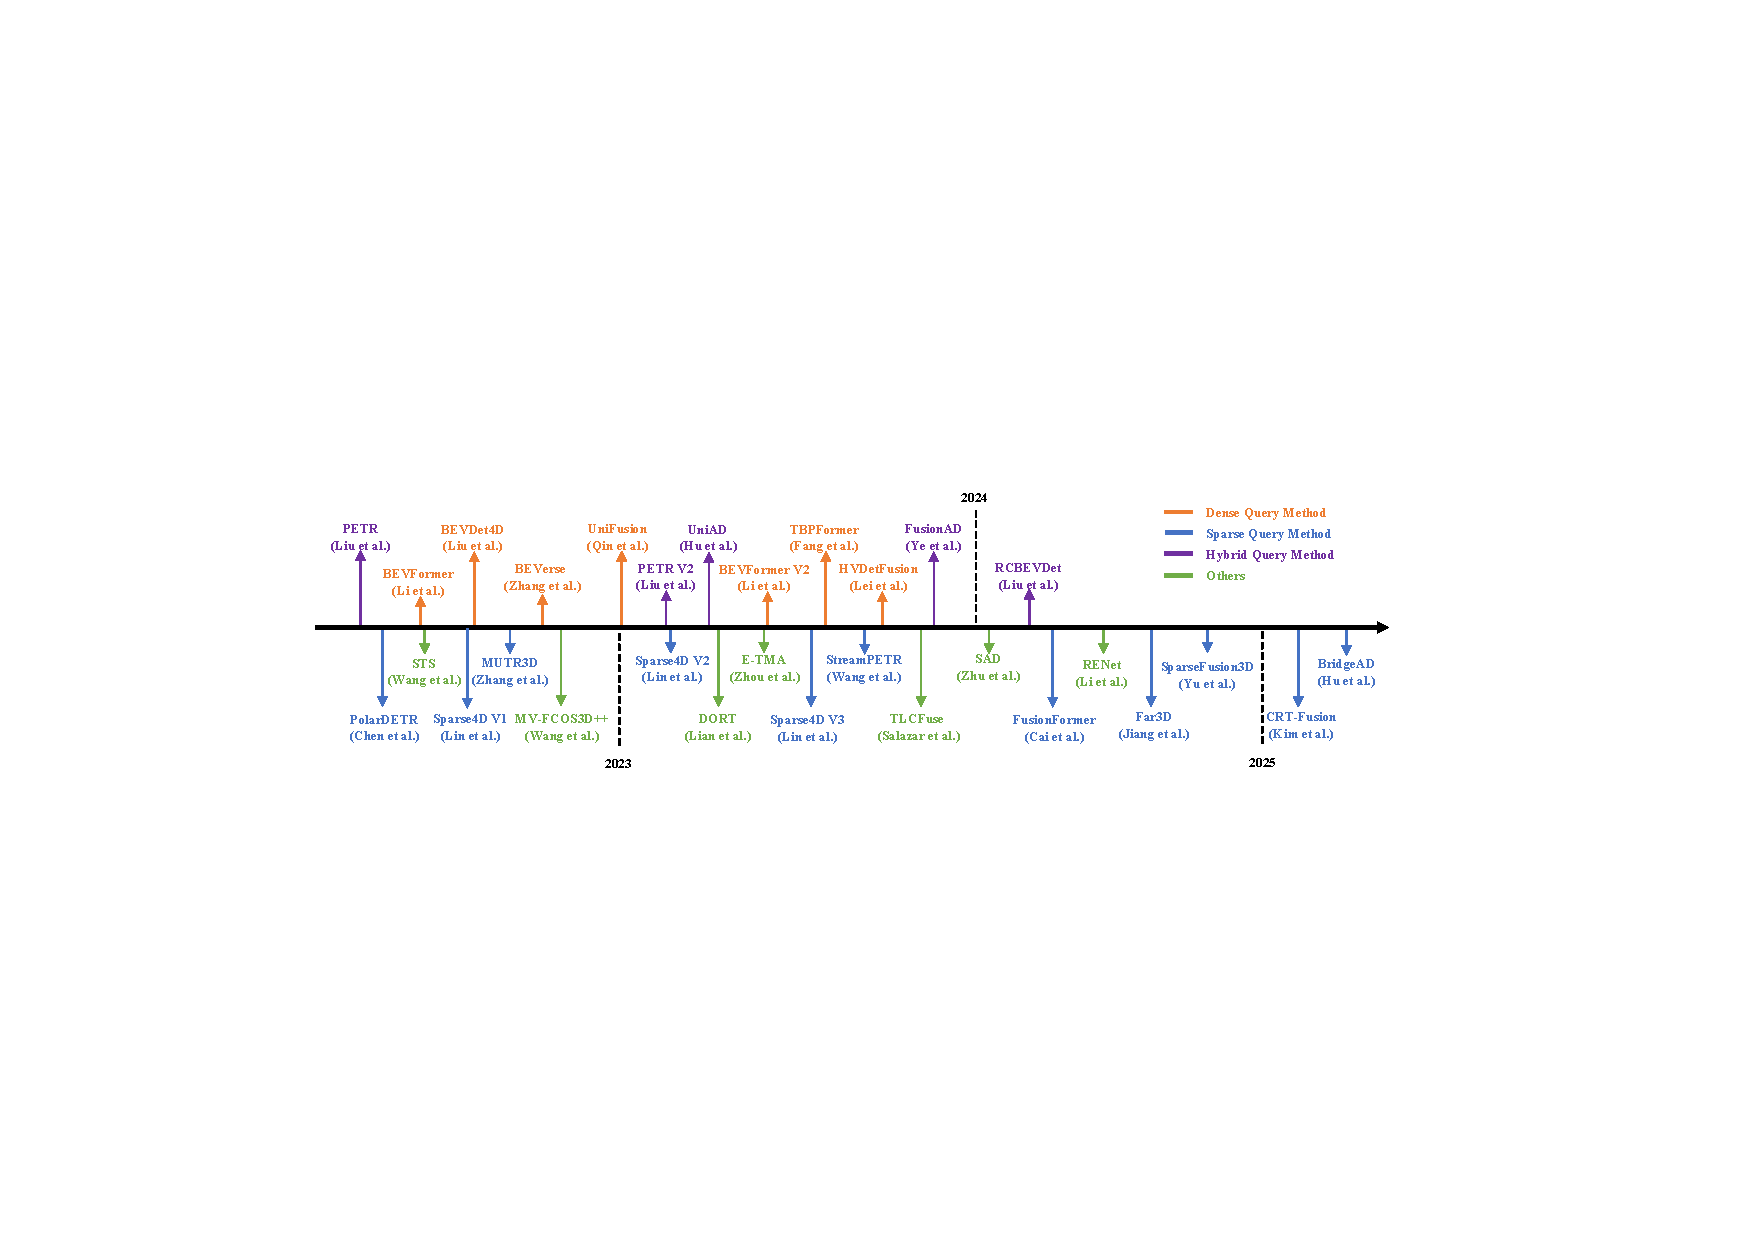
\includegraphics[width=180mm]{figure/time-series-timeline.pdf}
    \caption{Часова лінія методів злиття часових рядів.}
    \label{f:time-series-timeline}
\end{figure*}

\subsection{Методи щільних запитів}
Методи щільних запитів призначають кожній точці-запиту фіксовану растеризовану просторову позицію у 3D-просторі високої роздільної здатності або BEV-просторі~\cite{10670223}.
Серед них особливо репрезентативними є щільні каркаси на основі BEV; BEVFormer~\cite{li2022bevformer} став основоположною моделлю BEV-сприйняття. На основі DETR~\cite{carion2020end} і Deformable DETR~\cite{zhu2021deformable}, BEVFormer досягає адаптивної взаємодії ознак з кількох камерних видів через механізми деформівної уваги. На відміну від декодера у DETR3D~\cite{detr3d}, який покладається на розріджені об'єктні запити, BEVFormer включає додатковий енкодер на основі щільних BEV-запитів для генерування щільних BEV-ознак, що полегшує задачі семантичної сегментації. BEVFormer зливає часову інформацію між моментами $t-1$ і $t$ через модуль Temporal Self-Attention у своєму енкодері, що можна інтерпретувати як реалізацію механізму деформівної уваги~\cite{zhu2021deformable}. Розвиваючи цю основу, BEVFormer v2~\cite{yang2023bevformer} приймає двостадійну архітектуру детектування, що інтегрує перспективне детектування з BEV-детектуванням. Це дає BEVFormer v2 змогу навчатися 3D-представленням сцени адаптивно через перспективне нагляд, без покладання на дорогі дані для попереднього навчання глибини.

На основі LSS~\cite{philion2020lift}, представника глибинно-орієнтованих ``знизу-вгору'' підходів, BEVDet4D~\cite{huang2022bevdet4d} розширює 3D-детектування на 4D-часовий домен. BEVDet~\cite{huang2021bevdet} дотримується парадигми LSS і пропонує каркас 3D-детектування мультивидових камер у BEV. Окрім того, BEVDet4D зберігає BEV-ознаки попереднього кадру і зливає їх з ознаками поточного кадру через просторове вирівнювання та конкатенацію. Для подолання впливу власного руху транспортного засобу автори запропонували метод компенсації его-руху на основі згорток і забезпечили точність вирівнювання ознак через допоміжне завдання. Як уніфікований каркас сприйняття і прогнозування, BEVerse~\cite{zhang2022beverse} генерує 4D-BEV-представлення з мультикамерних відеопослідовностей через спільні модулі екстракції та підняття ознак.

Існують також методи з унікальними архітектурними рішеннями або оптимізаціями під конкретні завдання. На основі~\cite{li2022bevformer,yang2023bevformer,huang2021bevdet,huang2022bevdet4d}, UniFusion~\cite{qin2023unifusion} пропонує уніфікований каркас часово-просторового злиття, вводячи поняття віртуальних видів. Історичні кадри розглядаються як додаткові камерні види з просторово-перетворювальними відношеннями, що полегшує паралельну обробку часової та просторової інформації.
На цій базі TBPFormer~\cite{fang2023tbp} зосереджується на загальнішому архітектурному дизайні, пропонуючи енкодер PoseSync BEV для вирівнювання та синхронізації ознак і проектуючи часовий пірамідальний трансформер для багатомасштабної екстракції ознак і прогнозування майбутнього стану. HVDetFusion~\cite{lei2023hvdetfusion} додатково підтримує радарну модальність і проектує двостадійну розчеплену архітектуру детектування на основі BEVDet4D~\cite{huang2022bevdet4d}. Він використовує послідовність із 16 кадрів (\textit{тобто} 8 історичних і 8 майбутніх) для екстракції та злиття ознак, суттєво підвищуючи точність детектування та оцінки швидкості рухомих об'єктів.


\subsection{Методи розріджених запитів}

У складних відкритих середовищах, коли часова інформація інтегрується у процес злиття, обсяг даних, які мережа обробляє, зростає. Крім того, для задач, що вимагають прийняття рішень у реальному часі, на швидкість виводу моделі мають накладатися суворі вимоги. Тому методи розріджених запитів, відомі своєю ефективністю, точністю та придатністю до задач розрідженого сприйняття, набули поширення в індустрії.
У методах щільного BEV-представлення проста деформація багатокадрових BEV-ознак до поточного кадру і їх конкатенація часто дає хороші результати. Однак у представленнях з розрідженими запитами таке явне злиття стає надзвичайно складним. Як наслідок, багато підходів вдаються до взаємодії кожної ознаки-запиту з багатокадровими ознаками зображень, що додає значні обчислювальні витрати. StreamPETR~\cite{streampetr} розв'язує це шляхом систематичного поширення довгострокової інформації між кадрами через об'єктні запити. Ця об'єктно-центрична парадигма часового моделювання уникає обчислювальних навантажень моделювання часових відношень у щільних BEV-ознаках.

Услід за StreamPETR подальші роботи досягли подальших покращень у представленні ознак та стратегіях вибірки.
Однак BEV-методи мають внутрішні компроміси між дальністю сприйняття, точністю та обчислювальною ефективністю, водночас не можучи безпосередньо виконувати 2D-завдання сприйняття у домені зображень.
На ці обмеження Sparse4D v1~\cite{2211.10581} відповідає, досягаючи ефективної просторово-часової екстракції ознак через 4D-семплінг ключових точок та ієрархічне злиття ознак.
На основі Sparse4D v1, Sparse4D v2~\cite{lin2023sparse4d} застосовує рекурентний підхід, використовуючи розріджені екземпляри для поширення часової інформації, уникаючи багатокадрової вибірки заради ефективнішого злиття ознак.
Розвиваючи це, Sparse4D v3~\cite{2311.11722} робить наступний крок, пропонуючи часове очищення екземплярів та оцінювання якості, що одночасно прискорює збіжність моделі та підвищує продуктивність.

Багатозадачне навчання відіграє важливу роль у різних задачах сприйводу. Спільне навчання кількох завдань може робити нейромережу громіздкою, але використання розріджених запитів пропонує елегантне рішення.
MUTR3D~\cite{zhang2022mutr3d} — перший наскрізний 3D-каркас багатоцільового трекінгу, що пов'язує детектування цілей з низхідними завданнями, як-от планування шляху та передбачення траєкторії, через 3D MOT, і пропонує механізм 3D track query, який може моделювати просторово-часову узгодженість цілей між кадрами.
На основі MUTR3D, PF-Track~\cite{pang2023standing} приймає каркас ``трекінг за допомогою уваги'' і узгоджено представляє трековані екземпляри в часі за допомогою об'єктних запитів. У випадку довготривалих перекриттів PF-Track підтримує позиції об'єктів і дозволяє повторну асоціацію через модуль Future Reasoning, який обробляє історичну інформацію та передбачає стійкі майбутні траєкторії на термін до 4 секунд.

Крім того, нещодавні дослідження демонструють тенденцію до вивчення нових парадигм розрідженого мультимодального часового злиття. Більш ранні методи, як FusionFormer~\cite{cai2024fusionformer}, зосереджувались на часовому злитті BEV-ознак для 3D-детектування об'єктів, використовуючи механізми деформівної уваги та залишкові структури для вирівнювання та злиття ознак.
Попри інтуїтивну привабливість методів на основі щільних BEV-ознак, більшість з них суттєво втрачає інформацію при обробленні інформації по осі Z.
Також на основі DETR~\cite{wang2022detr3d}, QTNet~\cite{hou2023query} запропонував нову парадигму часового злиття, що використовує розріджені запити. Модуль моделювання часу, керованого рухом (motion-guided timing modeling, MTM), ефективно опрацьовує крос-модальну кореляцію між хмарами точок та ознаками зображень, досягаючи кращої продуктивності при збереженні легкої архітектури. SparseFusion3D~\cite{10314799} розвиває цей підхід, вводячи модуль MSPCP для передбачення зсуву хмари точок та інтегруючи стратегію ініціалізації запитів за допомогою радара для подолання виклику розрідженості. Еволюція від MTM (QTNet) до MSPCP (SparseFusion3D) представляє технологічний зсув від простого вирівнювання ознак до явного моделювання на основі руху. Модуль SQS у SparseFusion3D представляє розвиток стратегій мультимодального злиття від простої конкатенації ознак до складніших стратегій, як-от адаптивне зважене злиття.
Крім того, CRT-Fusion~\cite{kim2024crt} вирішує задачу врахування руху об'єктів у часовому злитті camera-radar шляхом введення багатокрокових запитів руху, що розрізняють кожен майбутній часовий крок. Метод використовує оцінювач ознак руху (Motion Feature Estimator) для передбачення піксельної швидкості та модуль Motion Guided Temporal Fusion для рекурентного вирівнювання ознак між часовими мітками, досягаючи переваг через явне врахування динаміки об'єктів.

\subsection{Методи гібридних запитів}
Методи гібридних запитів поєднують парадигми щільних і розріджених запитів, балансуючи обчислювальну ефективність із комплексним розумінням сцени. Ці підходи стратегічно використовують розріджені запити для об'єктних задач, водночас зберігаючи щільні представлення для просторово-повних задач, досягаючи оптимальної продуктивності у багатоцільових задачах сприйняття.

UniAD~\cite{hu2023planning} ілюструє цю гібридну архітектуру, інтегруючи сприйняття, прогнозування та планування в уніфікованому каркасі. Він використовує розріджені об'єктні запити для ефективного детектування і трекінгу, водночас зберігаючи щільні BEV-ознаки для прогнозування траєкторій і завдань планування. Це подвійне представлення забезпечує комплексне розуміння сцени без жертви продуктивності в реальному часі.
Розвиваючи успіх UniAD, FusionAD~\cite{ye2023fusionad} розширює гібридний підхід на мультимодальне часове злиття. Він обробляє дані камер та LiDAR через архітектуру на основі трансформерів, яка адаптивно перемикається між розрідженими та щільними представленнями залежно від вимог завдання, демонструючи гнучкість гібридних методів запитів у роботі з гетерогенними сенсорними даними.

Мультимодальні методи гібридних запитів, що ефективно опрацьовують гетерогенні дані з кількох сенсорів (різні кругові відеокамери або мультимодальні сенсори, \textit{напр.}, 4D-радар міліметрового діапазону, LiDAR, камера) через вишукані архітектури, демонструють чудові здатності у часово-просторовій екстракції та злитті ознак.
Спираючись на CRN~\cite{kim2023crn}, RCBEVdet~\cite{lin2024rcbevdet} вводить двопотокову мережу. Для радарного потоку проектується RadarBEVNet, що генерує щільні BEV-ознаки, для екстракції BEV-ознак з хмар точок.
Для камерного потоку використовується image backbone та трансформер виду з LSS~\cite{philion2020lift} для представлення ознак.
Далі, через модуль багаторівневого злиття на основі перехресної уваги (на базі deformable DETR), можна краще здійснити ефективне злиття 4D-радар міліметрового діапазону з камерою.

\section{Методи злиття MM-LLM}
\label{s:MM-LLM}

\begin{table}[t]
    \centering
    \caption{Класифікація методів злиття MM-LLM для MSFP.}
    \label{t:MM-LLM}
    \begin{tabular}{m{2cm}|m{2.8cm}|m{2.8cm}}
       \hline
       \textbf{Категорія}  & \textbf{Особливість} & \textbf{Методи} \\ \hline
        Візуально-мовні & Поєднують візуальні та текстові дані для семантичного вирівнювання.
        & Scedrivex~\cite{zhao2025sce2drivex}, X-Driver~\cite{liu2025x}, Mpdrive~\cite{zhang2025mpdrive}, SafeAuto~\cite{zhang2025safeauto}\\ \hline
        Візуально-LiDAR-мовні & Інтегрують візуальні, LiDAR- та мовні дані для 3D-просторового розуміння. & DriveMLM~\cite{wang2023drivemlm}, MAPLM~\cite{cao2024maplm}, LiDAR-LLM~\cite{yang2025lidar} \\ \hline
    \end{tabular}
\end{table}

\begin{figure}[t]
    \centering
    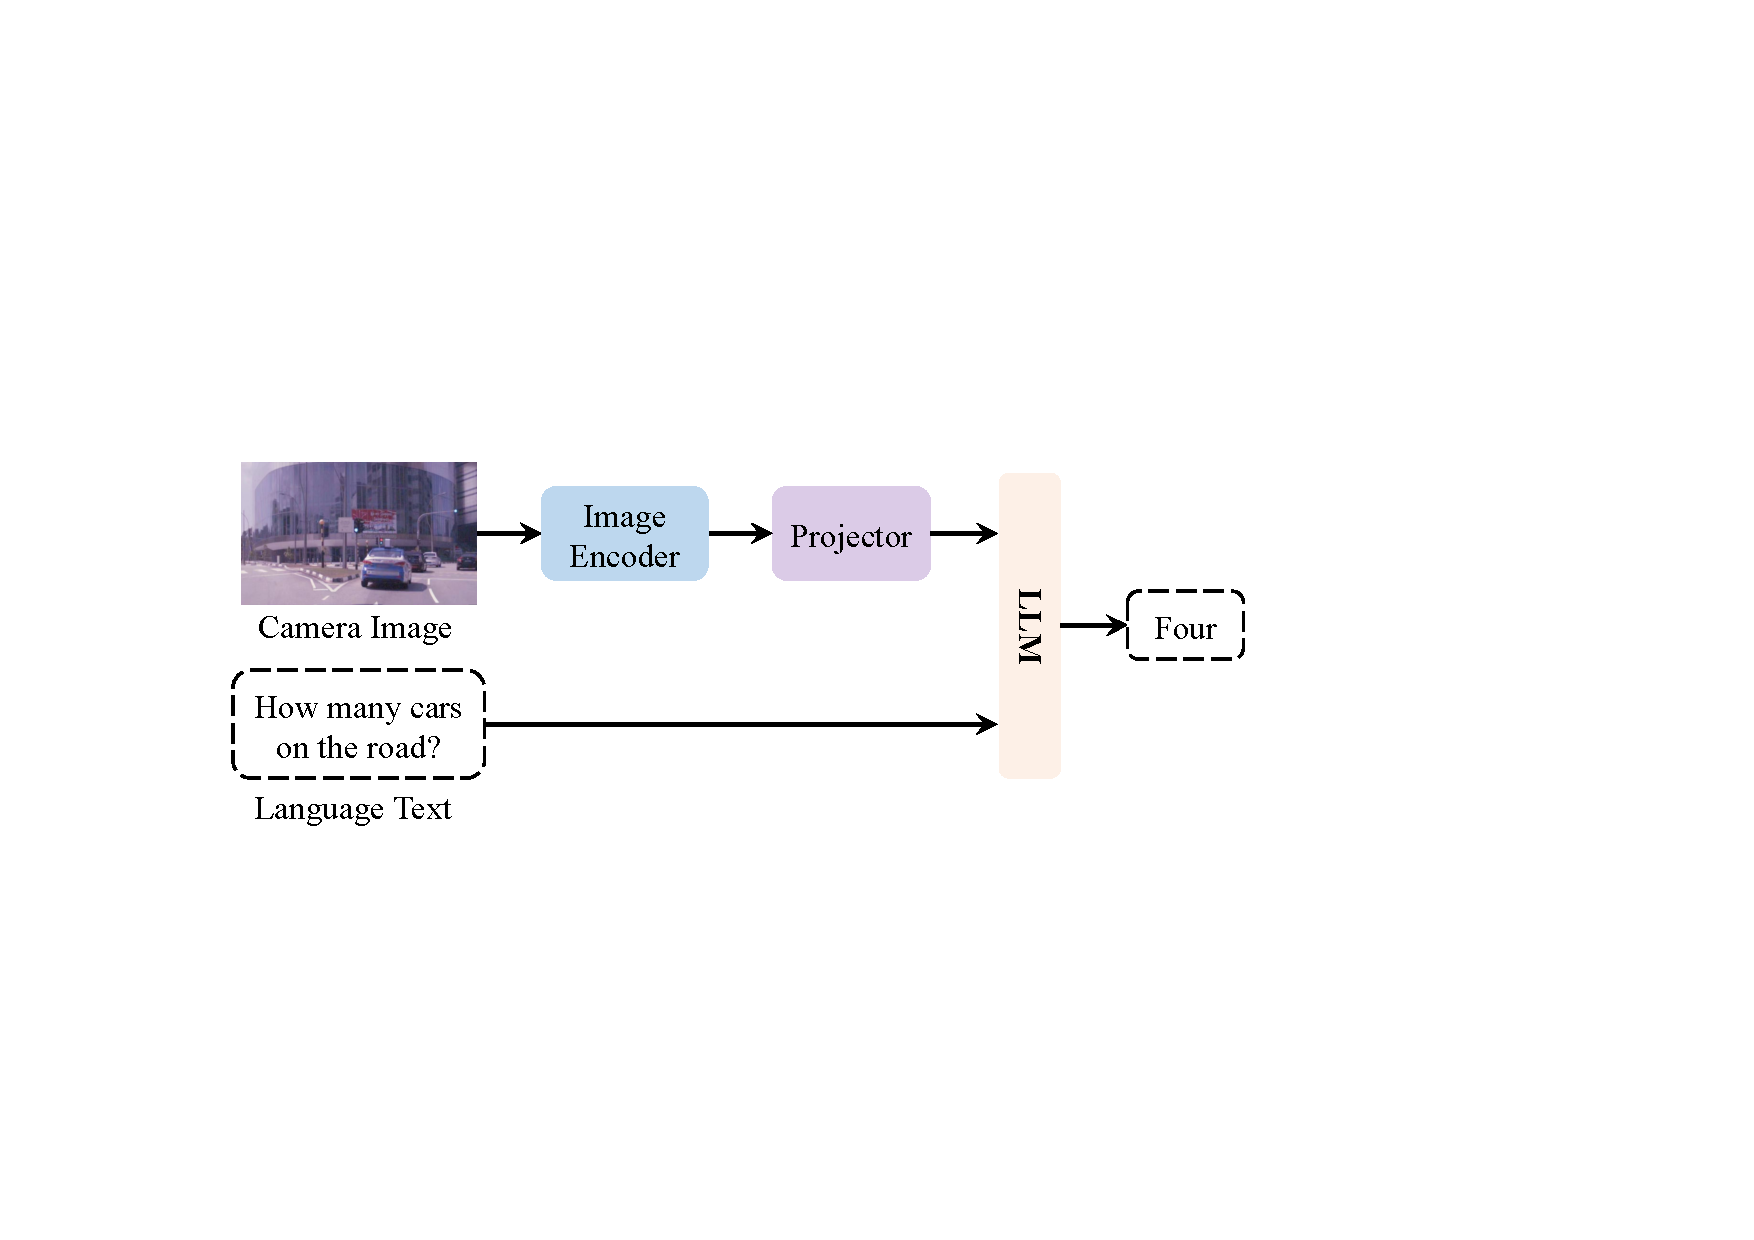
\includegraphics[width=85mm]{figure/Visual_Language-LLM.pdf}
    \caption{Парадигма на основі ``візуально-мовних'' методів.}
    \label{f:Visual-Language-LLM}
\end{figure}

В останні роки великі мовні моделі~(large language model, LLM) досягли вражаючої продуктивності у різноманітних задачах. Зливаючи дані з різних модальностей, мультимодальні LLM~(MM-LLM) можуть виконувати складніші завдання, як-от описи зображень, розуміння відео та крос-модальний пошук.
Останнім часом розроблено різноманітні нові набори даних задля просування MM-LLM для втіленого ШІ.
Наприклад, такі проєкти, як DriveLM~\cite{sima2023drivelm}, OmniDrive~\cite{wang2024omnidrive} та NuInstruct, збагачують наявні набори даних, включаючи LLM для генерації пар запитання-відповідь, що покривають сприйняття, міркування та планування.
Крім того, MAPLM~\cite{cao2024maplm} інтегрує мультивидові зображення з даними LiDAR для аналізу та інтерпретації станів дорожнього покриття.
На основі MM-LLM і цих наборів даних проведено багато досліджень щодо інтеграції MM-LLM до MSFP.
Як показано в табл.~\ref{t:MM-LLM}, у цьому розділі ми переважно розглядаємо існуючі споріднені роботи з двох категорій: \textit{методи на основі візуально-мовних моделей} та \textit{методи на основі візуально-LiDAR-мовних моделей}. Конвеєри цих двох категорій ілюструють відповідно рис.~\ref{f:Visual-Language-LLM} та рис.~\ref{f:Visual-LiDAR-LLM1}.



\subsection{Методи на основі візуально-мовних моделей}

Мультимодальні великі моделі демонструють значний потенціал у завданнях інтелектуального сприйняття; різні підходи досліджують їхні можливості для розв'язання складнощів реальних середовищ.
X-Driver~\cite{liu2025x} пропонує уніфікований каркас, який використовує мультимодальні великі мовні моделі з ланцюговим міркуванням (Chain-of-Thought) та авторегресійним моделюванням, досягаючи кращої продуктивності для автономного водіння у замкненому контурі та посиленої інтерпретованості.
Mpdrive~\cite{zhang2025mpdrive} вводить новий каркас підказкового навчання на основі маркерів, що використовує лаконічні візуальні маркери для представлення просторових координат і будує двозернисті візуальні підказки, досягаючи передових результатів зі збагаченим просторовим сприйняттям у задачах, що вимагають розвинутого просторового розуміння.
DriveVLM~\cite{tian2024drivevlm} інтегрує традиційні архітектури з MM-LLM через дві окремі гілки: одна зосереджена на традиційній візуальній обробці, інша використовує потужність мультимодальних трансформерів для розуміння сцени.

\begin{figure*}[t]
    \centering
    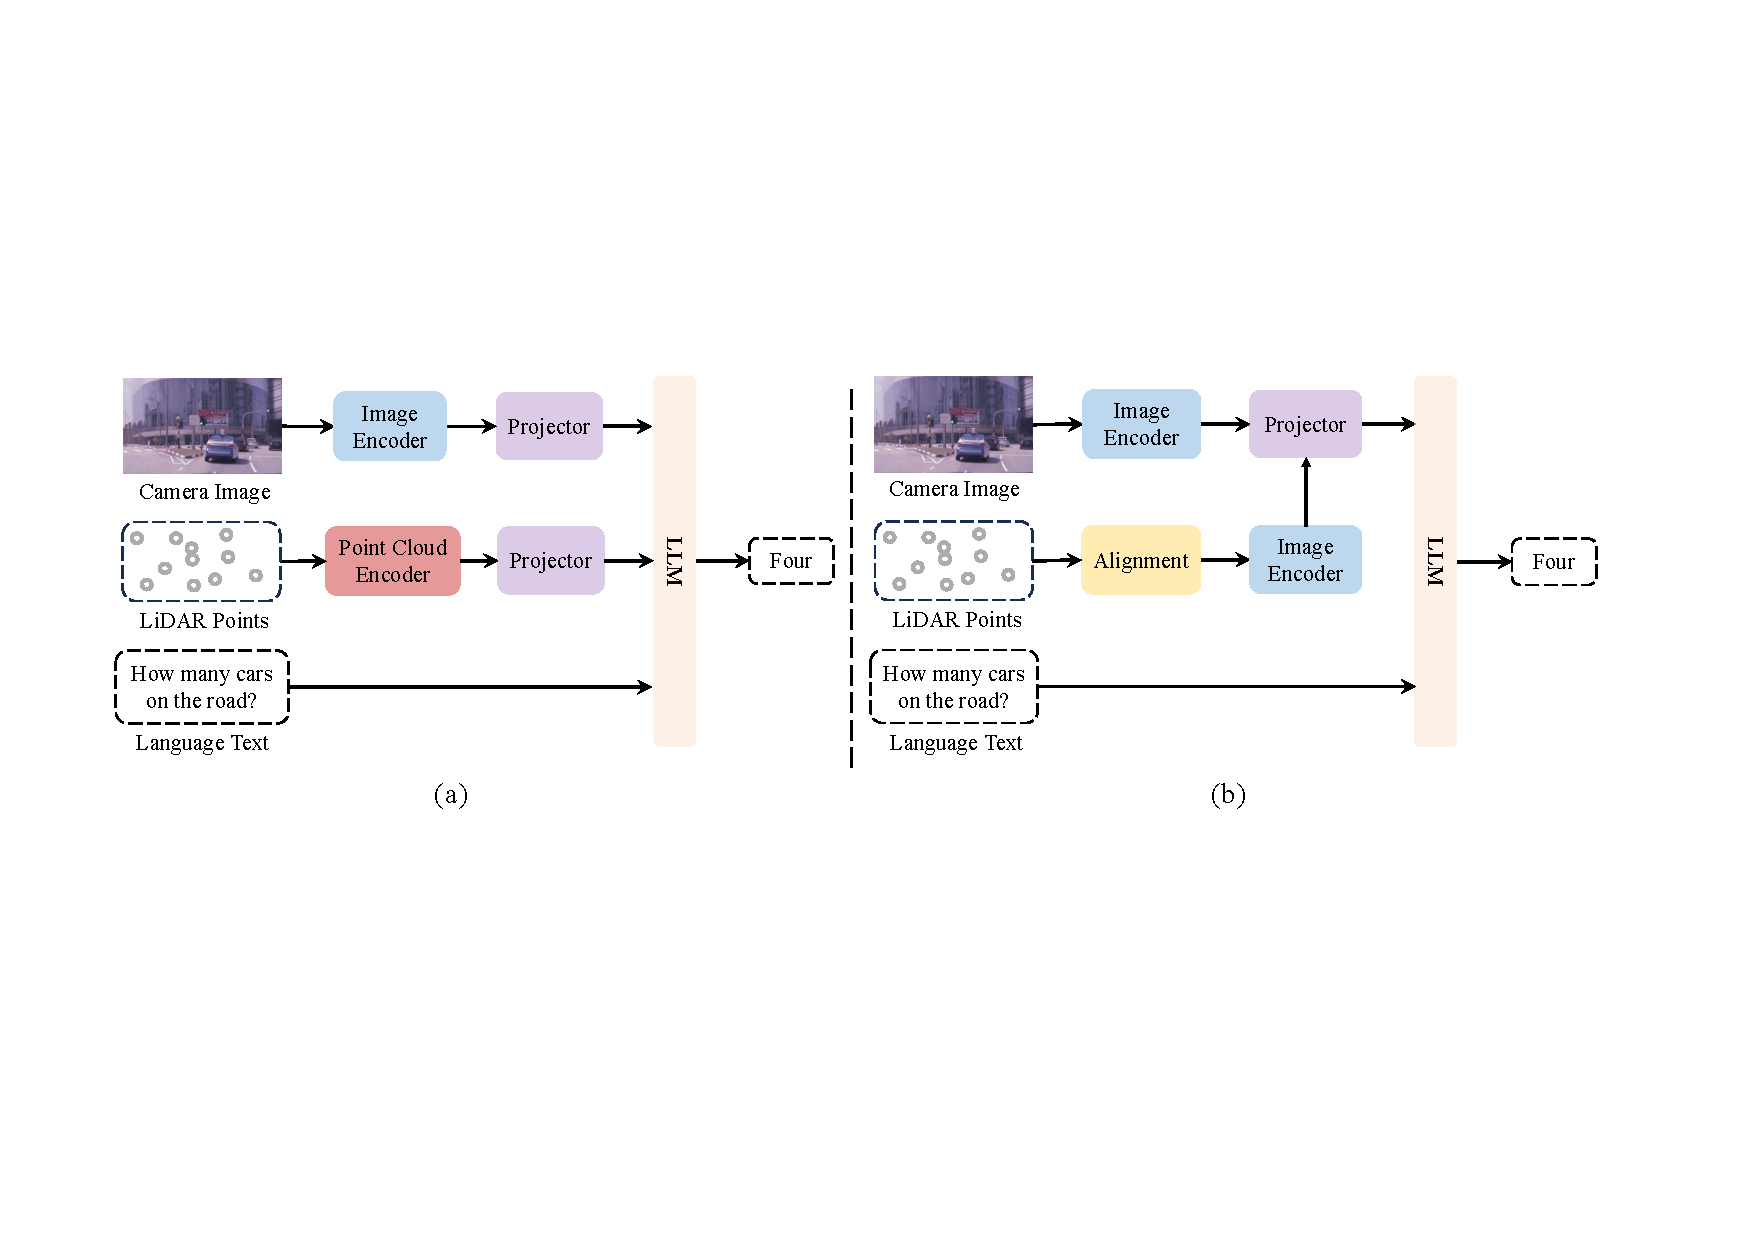
\includegraphics[width=180mm]{figure/visual-lidar-MMLLM.pdf}
    \caption{Парадигми на основі ``візуально-LiDAR-мовних'' моделей. У парадигмі~(а) проектуються окремі енкодери для радара і зображення, потім відбувається їх злиття. Парадигма~(б) зливає радарну хмару точок із зображенням після вирівнювання модальностей зображення.}
    \label{f:Visual-LiDAR-LLM1}
\end{figure*}

Поступ у проектуванні моделей надалі підвищує здатності сприйняття та міркування. Reason2Drive~\cite{nie2025reason2drive} використовує апріорний токенізатор для витягання локальних ознак зображення; BEV-InMLLM~\cite{ding2024holistic} вводить BEV-представлення для просторового розуміння; OmniDrive~\cite{wang2024omnidrive} інтегрує 2D попередньо натреновані знання з 3D-просторовими даними через Q-Former3D.
Тим часом ELM~\cite{zhou2025embodied} захоплює часову інформацію через механізм вибору токенів, що враховує час. Крім того, Chen \textit{et al.}~\cite{chen2024driving} пропонують нову архітектуру, що зливає об'єктно-рівневі векторизовані числові модальності в будь-який LLM за допомогою двостадійного методу попереднього тренування та тонкого налаштування.

\subsection{Методи на основі візуально-LiDAR-мовних моделей}

Через обмежену доступність даних LiDAR і текстових даних, безпосереднє вирівнювання ознак хмари точок з ознаками тексту є істотним викликом. Ця складність виникає тому, що дані хмари точок, що внутрішньо тривимірні й розріджені, не мають щільної та структурованої природи текстових даних. Щоб подолати ці виклики, ознаки зображення зазвичай використовуються як посередник для ефективного перекидання містка між текстом і LiDAR-даними.
Таким чином, багату візуальну інформацію, доступну в зображеннях, можна використати для безшовнішої інтеграції цих різнорідних типів даних.
У цьому напрямку,
DriveMLM~\cite{wang2023drivemlm} застосовує часовий QFormer для обробки мультивидових зображень, що дозволяє ефективно захоплювати часову динаміку та просторові зв'язки між різними перспективами. Це необхідно для розуміння складних сцен.

Крім того, у мультимодальній обробці деякі методи застосовують непрямий підхід до роботи з хмарами точок: вони перетворюють хмари точок на зображення для полегшення витягання інформації.
Таке перетворення дозволяє використати усталені техніки, що відзначаються в обробці зображень, тим самим підвищуючи загальну ефективність MSFP.
Наприклад, MAPLM~\cite{cao2024maplm} проектує 3D-хмару точок LiDAR на BEV-зображення, а ознаки витягає через візуальний енкодер.
Цей підхід перетворює 3D-дані на 2D-представлення, що полегшує обробку традиційними моделями глибокого навчання, призначеними для зображень. Використовуючи BEV-зображення, MAPLM перекидає міст між даними хмар точок і даними зображень, дозволяючи застосовувати потужні візуальні моделі, як-от CLIP.
Крім того, LiDAR-LLM~\cite{yang2025lidar} вводить нову схему розуміння 3D-сцен на відкритому повітрі, переформульовуючи 3D-когніцію як задачу мовного моделювання; використовується позиційно-усвідомлений трансформер (Position-Aware Transformer, PAT) та триетапна стратегія тренування для подолання модальнісної прогалини 3D-мова та досягнення передових результатів у задачах 3D-описів, прив'язки та відповідей на запитання.

\section{Відкриті виклики та майбутні можливості}
\label{s:open challenges}

У цьому розділі ми описуємо властиві виклики та можливі майбутні можливості для MSFP.
Обговорення нижче ведеться на трьох взаємопов'язаних рівнях: даних, моделі та застосування.


\subsection{Рівень даних}

\subsubsection{Якість даних}

Основний виклик на рівні даних — обмежена якість та репрезентативність наявних наборів даних для багатосенсорного злиття.
Багато наборів даних, як-от KITTI, nuScenes та Waymo Open, страждають на ``довгохвостові'' розподіли~\cite{geiger2012kitti, caesar2020nuscenes, sun2020waymo}.
Така незбалансованість обмежує здатність моделей злиття узагальнюватися до рідкісних, але критичних сценаріїв.
Більш того, попри збільшення різноманітності сенсорів, розрідженіші радарні хмари точок також ставлять виклик здатностям існуючих моделей до екстракції ознак. Це поглиблюється такими проблемами, як відсутні дані, викиди, зсуви (bias) і дрейф, а також відсутність стандартизованих методів оцінювання та обмежена доступність публічних наборів даних~\cite{teh2020sensor}.

Тому розвиток високоякісних наборів даних є істотним для розв'язання цих викликів.
Техніки AIGC (Artificial Intelligence Generated Content) потенційно можуть генерувати синтетичні дані для заповнення прогалин у наборах реальних даних, особливо для рідкісних або різноманітних сценаріїв, \textit{напр.}, фотореалістичний рендеринг~\cite{yangreal} і дифузійні моделі~\cite{croitoru2023diffusion}.
Для підвищення надійності згенерованих синтетичних даних майбутні дослідження могли б зосередитися на розробці автоматизованих інструментів виявлення помилок~\cite{ehrlinger2022survey}. Крім того, впровадження кількісних метрик якості може допомогти виявляти проблеми, як-от відсутні дані, викиди та дрейф даних.



\subsubsection{Аугментація даних}

Аугментація даних відіграє життєво важливу роль у підвищенні стійкості та узагальнюваності систем MSFP.
Однак мультимодальна аугментація даних також вносить унікальні виклики, зокрема в збереженні синхронізації між різними сенсорними модальностями~\cite{wang2021pointaugmenting, rangesh2021predicting}.
Беручи злиття LiDAR-камера як приклад: при застосуванні поворотів або зсувів до хмари точок LiDAR еквівалентні перетворення необхідно застосувати й до відповідних зображень камери для збереження просторової узгодженості~\cite{xiao2022polarmix}. Будь-які невідповідності в перетвореннях можуть зруйнувати просторові відношення між модальностями, що є вирішальним для ефективного злиття сенсорів.

Щоб подолати ці виклики, дослідники могли б зосередитися на розробці передових технік синхронізованої аугментації даних, адаптованих до систем MSFP. Один із потенційних напрямків досліджень — використання крос-модальних геометричних обмежень для забезпечення просторової узгодженості під час аугментації~\cite{yuan2023camera}.
Наприклад, перетворення хмари точок LiDAR можна поєднати з гомографічними перетвореннями у зображеннях камери, щоб зберегти точні просторові відношення.
Інший перспективний напрямок — AIGC, як-от дифузійні моделі~\cite{croitoru2023diffusion}, які можуть створювати реалістичні й синхронізовані аугментації для моделювання таких варіацій, як шум сенсорів і зміни середовища, при збереженні крос-модальної узгодженості.


\subsection{Рівень моделі}

\subsubsection{Ефективні стратегії злиття}

На рівні моделі розробка ефективних стратегій злиття передбачає подолання втрати інформації під час вирівнювання та інтеграції мультимодальних сенсорних даних. Втрата інформації часто виникає в процесі вирівнювання через невідповідності між сенсорними модальностями — наприклад, камери та LiDAR — які відрізняються фізичною конфігурацією, роздільною здатністю та перспективою~\cite{meyer2019sensor}. Фактори, як-от погода і освітлення, посилюють ці розбіжності, ускладнюючи точну синхронізацію~\cite{zhang2023perception}. Традиційні методи вирівнювання, як-от проектування хмар точок у систему координат камери~\cite{zhong2021survey}, часто вносять додаткові помилки, що ведуть до субоптимальної інтеграції.
Процеси інтеграції, як-от агрегація ознак, також додають до втрати інформації, стискаючи сенсорні дані та упускаючи критичні деталі. Наприклад, перетворення хмар точок у 2D-проекції (як-от BEV або range view) зменшує тривимірну просторову інформацію, як-от висоту, що життєво важлива для захоплення геометрії сцени~\cite{zhao2024bev, chang2023bev}. Ця сукупна втрата зменшує здатність моделі повноцінно використати взаємодоповнювальні переваги різних сенсорів, обмежуючи загальну продуктивність.

Щоб пом'якшити ці виклики, майбутні дослідження могли б зосередитися на стратегіях злиття, що спільно оптимізують точність вирівнювання та злиття даних. Техніки злиття з кількома представленнями, як-от поєднання воксельних ґраток, хмар точок і 2D-проекцій, відкривають шлях до збереження просторового та семантичного багатства~\cite{xu2021voxel}. Контекстно-усвідомлені підходи, що використовують часову узгодженість~\cite{zhu2024temporally}, та методи адаптивного навчання~\cite{lubken2024adaptive} можуть покращити вирівнювання через динамічну реакцію на зміни середовища. Крім того, механізми уваги~\cite{vaswani2017attention} можуть вибірково підкреслювати критичні ознаки кожної модальності під час інтеграції.
Більше того, такі техніки, як самоконтрольоване представницьке навчання~\cite{ericsson2022self} і контрастне навчання~\cite{wickstrom2022mixing}, мають потенціал захоплювати й використовувати крос-модальні зв'язки, надаючи багатшого й детальнішого нагляду для уточнення точності вирівнювання.
Ці рішення є основою для зменшення втрати інформації та підвищення стійкості мультимодальних систем злиття.


\subsubsection{Підхід на основі MM-LLM}

MM-LLM можна використати для обробки та злиття даних з різноманітних джерел — тексту, зображень і сенсорних виходів — що може значно збагатити розуміння складних середовищ~\cite{ye2024mplug, tiantokenize}.
Однак інтеграція цих моделей у реальні застосування втіленого ШІ все ще ставить критичні виклики.
Істотний виклик — робота з розрідженими та нерегулярними сенсорними даними, як-от хмари точок LiDAR і радара.
Висока вимірність даних радарних хмар точок вимагає вишуканих технік попередньої обробки та екстракції ознак для перетворення їх на формат, придатний для входу моделі. Крім того, радарні дані за своєю природою розріджені й неструктуровані, що ускладнює їх обробку порівняно зі структурованішими типами даних, як-от зображення чи текст~\cite{schumann2021radarscenes, li2020deep}.
Щоб подолати цю прогалину, майбутні дослідження могли б досліджувати гібридні архітектури, які поєднують техніки геометричного навчання — як-от графові нейромережі або моделі точкового навчання~\cite{svenningsson2021radar,murray2024estimating} — з мультимодальними здатностями MM-LLM.

Крім того, зовнішні знання MM-LLM, навчених на різноманітних наборах даних, можуть конфліктувати зі специфічними вимогами втіленого ШІ.
Наприклад, MM-LLM може зробити висновок, що сценарій із завантаженим пішохідним переходом застосовний універсально, пропонуючи зайві зупинки в середовищах, як-от шосе, де пішохідні переходи нерелевантні.
Такі конфлікти між загальними знаннями та специфічними контекстами можуть скомпрометувати прийняття рішень, якщо ними обережно не керувати або не адаптувати їх.
Щоб подолати ці виклики, майбутні дослідження могли б досліджувати такі механізми, як Retrieval-Augmented Generation (RAG), для динамічної адаптації зовнішніх знань до контексту, наданого багатосенсорними даними~\cite{sharifymoghaddam2024unirag}. Механізми уваги можуть додатково уточнювати цей процес, акцентуючи релевантну інформацію та відфільтровуючи нерелевантний або вводячий в оману контент.
Ці підходи надають потенційний шлях до забезпечення того, щоб зовнішні знання узгоджувалися зі специфічними реалчасовими вимогами систем втілених агентів, підвищуючи їхню стійкість і надійність.

\subsection{Рівень застосування}

\subsubsection{Адаптивність до реального світу}

У реальних відкритих середовищах умови суттєво змінюються: змінюються освітлення, погода та схеми руху. Раптові зміни — дощ, туман, сніг або перехід від дня до ночі — становлять істотні виклики для мультимодальних систем злиття, які повинні постійно підтримувати надійну продуктивність попри ці динамічні зміни.
Тому ефективна адаптація до різноманітних сценаріїв є істотною для забезпечення стійкості систем MSFP і запобігання відмовам у складних умовах.


Щоб покращити адаптивність до реального світу, майбутні дослідження могли б зосередитися на розробці самоадаптивних алгоритмів, що можуть налаштовувати параметри моделі у відповідь на зміни середовища в реальному часі~\cite{xing2024comprehensive}.
Такі техніки, як адаптація доменів та онлайн-навчання~\cite{silva2023adaptive, hoi2021online}, дозволяють моделям підтримувати продуктивність, постійно адаптуючись до нових розподілів даних без перетренування з нуля.
Крім того, можна досліджувати методи zero-shot learning~\cite{wang2019survey, xian2018zero}, що дозволяють моделям узагальнюватися до невидимих сценаріїв і опрацьовувати нові умови середовища без попереднього специфічного тренування, поліпшуючи їхню здатність впоратися з непередбачуваними реальними ситуаціями.


\subsubsection{Інтерпретованість (Explainability)}

Інтерпретованість суттєво важлива для моделей MSFP у втіленому ШІ, оскільки вона будує довіру, забезпечує прозорість і допомагає в налагодженні, особливо в безпеково-критичних застосуваннях~\cite{de2024building}.
Один з основних викликів полягає у виявленні внеску кожної сенсорної модальності у різних умовах.
Наприклад, LiDAR може грати ключову роль у поганому освітленні, тоді як камери можуть бути ефективнішими за ясної погоди.
Розуміння цих внесків — а також того, як різні модальності взаємодіють — складне, оскільки ці відношення часто не прямі, особливо у складних реальних сценаріях.

Майбутні дослідження могли б досліджувати методи контекстно-усвідомленої інтерпретованості~\cite{wang2023context} для прояснення ролі кожної модальності залежно від умов середовища та стадій злиття.
Наприклад, інструменти візуалізації на основі уваги~\cite{jin2022visual, yeh2023attentionviz} можуть підкреслити, які сенсори зробили найбільший внесок у конкретних сценаріях, підвищуючи прозорість прийняття рішень.
Крім того, можна проектувати інтерпретовані мережі злиття, що видають специфічні для модальності оцінки впевненості, надаючи чітке розуміння того, як кожне джерело даних вплинуло на вихід, особливо в критичних або неоднозначних ситуаціях.
Адаптація пояснень до модальностей та сценаріїв застосування може посилити довіру користувача та підтримати безпечніше й ефективніше розгортання у реальних середовищах.

\section{Висновок}
\label{s:conclusion}

У цьому огляді ми всебічно розглянули методи досліджень багатосенсорного сприйняття на основі злиття даних~(MSFP) для втіленого ШІ.
Зокрема, ми спочатку ввели передумови MSFP.
Далі впорядкували й розглянули конкретні методи за чотирма категоріями: методи мультимодального злиття, мультиагентного злиття, злиття часових рядів та злиття MM-LLM.
Нарешті, обговорили поточні виклики та майбутні можливості.
Озираючись назад: на відміну від існуючих оглядів, що зосереджуються на конкретних областях~(\textit{напр.}, автономне керування) або задачах~(\textit{напр.}, 3D-детектування об'єктів), ми впорядкували дослідження MSFP з \emph{незалежної від завдання} перспективи, де методи представлено суто з різних технічних точок зору.
Тому ця стаття придатна для прочитання дуже широкого кола дослідників, у різних областях і з різних задач.
У майбутньому ми регулярно оновлюватимемо цей огляд онлайн, щоб подавати найсвіжіший передовий поступ у галузі MSFP.

З огляду на обмежену експертизу авторів, якщо у статті є якісь недоліки, просимо повідомляти. Ми серйозно покращимо огляд у наступній версії.


\bibliographystyle{IEEEtran}
\bibliography{ref}

\vfill

\end{document}
